\documentclass[10pt]{beamer}

\usepackage[T1]{fontenc}

\usetheme{metropolis}

\usepackage{graphicx}
\graphicspath{{images/}}
\usepackage{amsmath, amssymb, amsthm}
\usepackage{mathtools}
\usepackage{bm}
\usepackage{booktabs}
\usepackage{caption}
\usepackage{array}
\usepackage{tikz}
\usetikzlibrary{positioning, arrows.meta, calc, fit, backgrounds, decorations.pathreplacing}
\usepackage{listings}
\usepackage{xcolor}
\usepackage[numbers,square]{natbib}
\usepackage[most]{tcolorbox}
\usepackage{tabularx}
\definecolor{codebg}{RGB}{245,245,245}
\definecolor{codeframe}{RGB}{180,180,180}
\definecolor{boxbg}{RGB}{235,245,255}
\definecolor{boxframe}{RGB}{70,130,180}
\definecolor{ctrl}{HTML}{EB6834}   % P.ORANGE: the control, as in the figures

\lstdefinestyle{pytorch}{
  language=Python,
  basicstyle=\ttfamily\scriptsize,
  keywordstyle=\color{blue!70!black}\bfseries,
  stringstyle=\color{green!50!black},
  commentstyle=\color{gray}\itshape,
  showstringspaces=false,
  breaklines=true,
  columns=fullflexible,
  backgroundcolor=\color{codebg},
  frame=single,
  rulecolor=\color{codeframe},
  framesep=4pt,
  xleftmargin=4pt,
  xrightmargin=4pt,
}
\lstset{style=pytorch}

\title{The Training Loop}
\subtitle{Mathematical Foundations of Control and Machine Learning}
\author{Enrique Zuazua, Daniel L\'opez Montero}
\date{Winter 2026}
\institute{FAU Erlangen-N\"urnberg}

% --- Math shortcuts --------------------------------------------------------
\newcommand{\R}{\mathbb{R}}
\newcommand{\N}{\mathbb{N}}
\newcommand{\E}{\mathbb{E}}
\newcommand{\Prob}{\mathbb{P}}
\newcommand{\Risk}{\mathcal{R}}    % the population risk; the empirical risk is F
\newcommand{\Gram}{\mathcal{G}}
\newcommand{\ctrl}[1]{\textcolor{ctrl}{#1}}
\DeclareMathOperator{\Range}{Range}
\DeclareMathOperator{\Var}{Var}
\DeclareMathOperator{\Cov}{Cov}
\DeclareMathOperator{\KL}{KL}
\DeclareMathOperator{\softmax}{softmax}
\DeclareMathOperator*{\argmin}{arg\,min}
\DeclareMathOperator*{\argmax}{arg\,max}

% --- A box for definitions and theorems ------------------------------------
\newtcolorbox{mathbox}[2][]{
  colback=boxbg, colframe=boxframe, boxrule=0.2pt, arc=2pt,
  left=4pt, right=4pt, top=2pt, bottom=2pt,
  title=\textbf{#2}, fonttitle=\small, coltitle=white, colbacktitle=boxframe,
  halign=left, #1}

% --- Notebook references for worked examples and exercises only ------------
\newcommand{\nbref}[1]{%
  \begin{tikzpicture}[remember picture, overlay]
    \node[anchor=south west, font=\scriptsize, text=black!55]
      at ([xshift=5mm, yshift=1.1mm] current page.south west) {Notebook #1};
  \end{tikzpicture}}

% --- The four steps of the lecture ------------------------------------------
% \loopdiagram{k} draws the loop with step k highlighted: 1 data, 2 architecture, 3 loss,
% 4 optimizer; 0 highlights nothing and 5 the whole loop.  It opens each part of the lecture.
\newcommand{\loopdiagram}[1]{%
\begin{tikzpicture}[x=1cm, y=1cm, font=\scriptsize, >=Stealth,
    loopstep/.style={draw=boxframe, fill=boxbg, rounded corners=2pt, align=center,
                     minimum width=2.22cm, minimum height=0.82cm, inner sep=2pt},
    loopon/.style={draw=ctrl, fill=ctrl!14, line width=0.9pt},
    looparrow/.style={->, boxframe, line width=0.7pt},
    loopA/.style={}, loopB/.style={}, loopC/.style={}, loopD/.style={}, loopE/.style={}]
  \ifcase#1\relax
  \or \tikzset{loopA/.style={loopon}}%
  \or \tikzset{loopB/.style={loopon}}%
  \or \tikzset{loopC/.style={loopon}}%
  \or \tikzset{loopD/.style={loopon}}%
  \or \tikzset{loopA/.style={loopon}, loopB/.style={loopon}, loopC/.style={loopon},
               loopD/.style={loopon}, loopE/.style={ctrl}}%
  \fi
  \node[loopstep, loopA] (loopdata) at (0,0)    {\textbf{1. Data}\\ representation $\varphi$};
  \node[loopstep, loopB] (looparch) at (2.62,0) {\textbf{2. Architecture}\\ model $f(\,\cdot\,;w)$};
  \node[loopstep, loopC] (looploss) at (5.24,0) {\textbf{3. Loss}\\ $\ell(f(x;w),y)$};
  \node[loopstep, loopD] (loopopt)  at (7.86,0) {\textbf{4. Optimizer}\\ $w_{k+1}=w_k-\eta\,g_k$};
  \draw[looparrow] (loopdata) -- (looparch);
  \draw[looparrow] (looparch) -- (looploss);
  \draw[looparrow] (looploss) -- (loopopt);
  \draw[looparrow, loopE] (loopopt.north) -- ++(0,0.32) -|
    node[pos=0.25, above, text=black!70, inner sep=1.5pt] {update the parameters $w$} (looparch.north);
\end{tikzpicture}}

\setbeamerfont{standout}{size=\Large, series=\mdseries}
\setbeamertemplate{bibliography item}[text]
\renewcommand{\bibsection}{}


% --- Bibliography database -------------------------------------------------
% The entries live here so that the slides are one self-contained file.  Each
% compilation writes them to the_training_loop.bib for BibTeX: edit this block,
% not the generated .bib file.
\begin{filecontents}[overwrite]{the_training_loop.bib}
@inproceedings{vaswani2017,
  author    = {Vaswani, Ashish and Shazeer, Noam and Parmar, Niki and Uszkoreit, Jakob and Jones, Llion and Gomez, Aidan N. and Kaiser, {\L}ukasz and Polosukhin, Illia},
  title     = {Attention Is All You Need},
  booktitle = {Advances in Neural Information Processing Systems 30},
  pages     = {5998--6008},
  year      = {2017}
}

@techreport{radford2019,
  author      = {Radford, Alec and Wu, Jeffrey and Child, Rewon and Luan, David and Amodei, Dario and Sutskever, Ilya},
  title       = {Language Models Are Unsupervised Multitask Learners},
  institution = {OpenAI},
  year        = {2019},
  url         = {https://cdn.openai.com/better-language-models/language_models_are_unsupervised_multitask_learners.pdf}
}

@inproceedings{brown2020,
  author    = {Brown, Tom B. and Mann, Benjamin and Ryder, Nick and Subbiah, Melanie and others},
  title     = {Language Models Are Few-Shot Learners},
  booktitle = {Advances in Neural Information Processing Systems 33},
  pages     = {1877--1901},
  year      = {2020}
}

@misc{grattafiori2024,
  author = {Grattafiori, Aaron and Dubey, Abhimanyu and Jauhri, Abhinav and Pandey, Abhinav and Kadian, Abhishek and Al-Dahle, Ahmad and others},
  title  = {The {Llama} 3 Herd of Models},
  year   = {2024},
  note   = {arXiv:2407.21783}
}

@inproceedings{sennrich2016,
  author    = {Sennrich, Rico and Haddow, Barry and Birch, Alexandra},
  title     = {Neural Machine Translation of Rare Words with Subword Units},
  booktitle = {Proceedings of the 54th Annual Meeting of the Association for Computational Linguistics (Volume 1: Long Papers)},
  pages     = {1715--1725},
  year      = {2016},
  doi       = {10.18653/v1/P16-1162}
}

@inproceedings{tancik2020,
  author    = {Tancik, Matthew and Srinivasan, Pratul P. and Mildenhall, Ben and Fridovich-Keil, Sara and Raghavan, Nithin and Singhal, Utkarsh and Ramamoorthi, Ravi and Barron, Jonathan T. and Ng, Ren},
  title     = {Fourier Features Let Networks Learn High Frequency Functions in Low Dimensional Domains},
  booktitle = {Advances in Neural Information Processing Systems 33},
  pages     = {7537--7547},
  year      = {2020},
  note      = {arXiv:2006.10739}
}

@inproceedings{dosovitskiy2021,
  author    = {Dosovitskiy, Alexey and Beyer, Lucas and Kolesnikov, Alexander and Weissenborn, Dirk and Zhai, Xiaohua and Unterthiner, Thomas and Dehghani, Mostafa and Minderer, Matthias and Heigold, Georg and Gelly, Sylvain and Uszkoreit, Jakob and Houlsby, Neil},
  title     = {An Image Is Worth 16x16 Words: Transformers for Image Recognition at Scale},
  booktitle = {International Conference on Learning Representations (ICLR)},
  year      = {2021},
  note      = {arXiv:2010.11929}
}

@inproceedings{rombach2022,
  author    = {Rombach, Robin and Blattmann, Andreas and Lorenz, Dominik and Esser, Patrick and Ommer, Bj{\"o}rn},
  title     = {High-Resolution Image Synthesis with Latent Diffusion Models},
  booktitle = {IEEE/CVF Conference on Computer Vision and Pattern Recognition (CVPR)},
  pages     = {10674--10685},
  year      = {2022},
  doi       = {10.1109/CVPR52688.2022.01042}
}

@misc{bronstein2021,
  author = {Bronstein, Michael M. and Bruna, Joan and Cohen, Taco and Veli{\v{c}}kovi{\'c}, Petar},
  title  = {Geometric Deep Learning: Grids, Groups, Graphs, Geodesics, and Gauges},
  year   = {2021},
  note   = {arXiv:2104.13478}
}

@article{rumelhart1986,
  author  = {Rumelhart, David E. and Hinton, Geoffrey E. and Williams, Ronald J.},
  title   = {Learning Representations by Back-Propagating Errors},
  journal = {Nature},
  volume  = {323},
  pages   = {533--536},
  year    = {1986},
  doi     = {10.1038/323533a0}
}

@article{lecun1998,
  author  = {LeCun, Yann and Bottou, L{\'e}on and Bengio, Yoshua and Haffner, Patrick},
  title   = {Gradient-Based Learning Applied to Document Recognition},
  journal = {Proceedings of the IEEE},
  volume  = {86},
  number  = {11},
  pages   = {2278--2324},
  year    = {1998},
  doi     = {10.1109/5.726791}
}

@inproceedings{he2016,
  author    = {He, Kaiming and Zhang, Xiangyu and Ren, Shaoqing and Sun, Jian},
  title     = {Deep Residual Learning for Image Recognition},
  booktitle = {IEEE Conference on Computer Vision and Pattern Recognition (CVPR)},
  pages     = {770--778},
  year      = {2016},
  doi       = {10.1109/CVPR.2016.90}
}

@article{elman1990,
  author  = {Elman, Jeffrey L.},
  title   = {Finding Structure in Time},
  journal = {Cognitive Science},
  volume  = {14},
  number  = {2},
  pages   = {179--211},
  year    = {1990},
  doi     = {10.1207/s15516709cog1402_1}
}

@book{minsky1969,
  author    = {Minsky, Marvin and Papert, Seymour},
  title     = {Perceptrons: An Introduction to Computational Geometry},
  publisher = {MIT Press},
  address   = {Cambridge, MA},
  year      = {1969}
}

@inproceedings{hastad1986,
  author    = {H{\aa}stad, Johan},
  title     = {Almost Optimal Lower Bounds for Small Depth Circuits},
  booktitle = {Proceedings of the 18th Annual ACM Symposium on Theory of Computing (STOC)},
  pages     = {6--20},
  year      = {1986},
  doi       = {10.1145/12130.12132}
}

@article{furst1984,
  author  = {Furst, Merrick and Saxe, James B. and Sipser, Michael},
  title   = {Parity, Circuits, and the Polynomial-Time Hierarchy},
  journal = {Mathematical Systems Theory},
  volume  = {17},
  number  = {1},
  pages   = {13--27},
  year    = {1984},
  doi     = {10.1007/BF01744431}
}

@article{ajtai1983,
  author  = {Ajtai, Mikl{\'o}s},
  title   = {{$\Sigma^1_1$}-Formulae on Finite Structures},
  journal = {Annals of Pure and Applied Logic},
  volume  = {24},
  number  = {1},
  pages   = {1--48},
  year    = {1983},
  doi     = {10.1016/0168-0072(83)90038-6}
}

@inproceedings{yao1985,
  author    = {Yao, Andrew Chi-Chih},
  title     = {Separating the Polynomial-Time Hierarchy by Oracles},
  booktitle = {26th Annual Symposium on Foundations of Computer Science (FOCS)},
  pages     = {1--10},
  year      = {1985},
  doi       = {10.1109/SFCS.1985.49}
}

@incollection{rumelhart1986pdp,
  author    = {Rumelhart, David E. and Hinton, Geoffrey E. and Williams, Ronald J.},
  title     = {Learning Internal Representations by Error Propagation},
  booktitle = {Parallel Distributed Processing: Explorations in the Microstructure of Cognition, Volume 1: Foundations},
  editor    = {Rumelhart, David E. and McClelland, James L.},
  publisher = {MIT Press},
  address   = {Cambridge, MA},
  pages     = {318--362},
  year      = {1986}
}

@misc{telgarsky2015,
  author = {Telgarsky, Matus},
  title  = {Representation Benefits of Deep Feedforward Networks},
  year   = {2015},
  note   = {arXiv:1509.08101}
}

@inproceedings{telgarsky2016,
  author    = {Telgarsky, Matus},
  title     = {Benefits of Depth in Neural Networks},
  booktitle = {29th Annual Conference on Learning Theory (COLT)},
  series    = {PMLR},
  volume    = {49},
  pages     = {1517--1539},
  year      = {2016}
}

@article{huber1964,
  author  = {Huber, Peter J.},
  title   = {Robust Estimation of a Location Parameter},
  journal = {The Annals of Mathematical Statistics},
  volume  = {35},
  number  = {1},
  pages   = {73--101},
  year    = {1964},
  doi     = {10.1214/aoms/1177703732}
}

@book{bishop2006,
  author    = {Bishop, Christopher M.},
  title     = {Pattern Recognition and Machine Learning},
  publisher = {Springer},
  address   = {New York},
  year      = {2006}
}

@article{gneiting2007,
  author  = {Gneiting, Tilmann and Raftery, Adrian E.},
  title   = {Strictly Proper Scoring Rules, Prediction, and Estimation},
  journal = {Journal of the American Statistical Association},
  volume  = {102},
  number  = {477},
  pages   = {359--378},
  year    = {2007},
  doi     = {10.1198/016214506000001437}
}

@techreport{bishop1994,
  author      = {Bishop, Christopher M.},
  title       = {Mixture Density Networks},
  institution = {Neural Computing Research Group, Aston University},
  address     = {Birmingham},
  number      = {NCRG/94/004},
  year        = {1994},
  url         = {https://publications.aston.ac.uk/id/eprint/373/}
}

@article{saito2015,
  author  = {Saito, Takaya and Rehmsmeier, Marc},
  title   = {The Precision-Recall Plot Is More Informative than the {ROC} Plot When Evaluating Binary Classifiers on Imbalanced Datasets},
  journal = {PLoS ONE},
  volume  = {10},
  number  = {3},
  pages   = {e0118432},
  year    = {2015},
  doi     = {10.1371/journal.pone.0118432}
}

@inproceedings{elkan2001,
  author    = {Elkan, Charles},
  title     = {The Foundations of Cost-Sensitive Learning},
  booktitle = {Proceedings of the 17th International Joint Conference on Artificial Intelligence (IJCAI)},
  pages     = {973--978},
  year      = {2001}
}

@inproceedings{lin2017,
  author    = {Lin, Tsung-Yi and Goyal, Priya and Girshick, Ross and He, Kaiming and Doll{\'a}r, Piotr},
  title     = {Focal Loss for Dense Object Detection},
  booktitle = {IEEE International Conference on Computer Vision (ICCV)},
  pages     = {2999--3007},
  year      = {2017},
  doi       = {10.1109/ICCV.2017.324}
}

@article{robbins1951,
  author  = {Robbins, Herbert and Monro, Sutton},
  title   = {A Stochastic Approximation Method},
  journal = {The Annals of Mathematical Statistics},
  volume  = {22},
  number  = {3},
  pages   = {400--407},
  year    = {1951},
  doi     = {10.1214/aoms/1177729586}
}

@inproceedings{li2017,
  author    = {Li, Qianxiao and Tai, Cheng and E, Weinan},
  title     = {Stochastic Modified Equations and Adaptive Stochastic Gradient Algorithms},
  booktitle = {Proceedings of the 34th International Conference on Machine Learning (ICML)},
  series    = {PMLR},
  volume    = {70},
  pages     = {2101--2110},
  year      = {2017}
}

@article{bottou2018,
  author  = {Bottou, L{\'e}on and Curtis, Frank E. and Nocedal, Jorge},
  title   = {Optimization Methods for Large-Scale Machine Learning},
  journal = {SIAM Review},
  volume  = {60},
  number  = {2},
  pages   = {223--311},
  year    = {2018},
  doi     = {10.1137/16M1080173}
}

@inproceedings{loshchilov2017,
  author    = {Loshchilov, Ilya and Hutter, Frank},
  title     = {{SGDR}: Stochastic Gradient Descent with Warm Restarts},
  booktitle = {International Conference on Learning Representations (ICLR)},
  year      = {2017},
  note      = {arXiv:1608.03983}
}

@inproceedings{smith2018,
  author    = {Smith, Samuel L. and Kindermans, Pieter-Jan and Ying, Chris and Le, Quoc V.},
  title     = {Don't Decay the Learning Rate, Increase the Batch Size},
  booktitle = {International Conference on Learning Representations (ICLR)},
  year      = {2018},
  note      = {arXiv:1711.00489}
}

@misc{goyal2017,
  author = {Goyal, Priya and Doll{\'a}r, Piotr and Girshick, Ross and Noordhuis, Pieter and Wesolowski, Lukasz and Kyrola, Aapo and Tulloch, Andrew and Jia, Yangqing and He, Kaiming},
  title  = {Accurate, Large Minibatch {SGD}: Training {ImageNet} in 1 Hour},
  year   = {2017},
  note   = {arXiv:1706.02677}
}

@inproceedings{devlin2019,
  author    = {Devlin, Jacob and Chang, Ming-Wei and Lee, Kenton and Toutanova, Kristina},
  title     = {{BERT}: Pre-training of Deep Bidirectional Transformers for Language Understanding},
  booktitle = {Proceedings of the 2019 Conference of the North American Chapter of the Association for Computational Linguistics: Human Language Technologies (NAACL-HLT)},
  pages     = {4171--4186},
  year      = {2019},
  doi       = {10.18653/v1/N19-1423}
}

@misc{hoffmann2022,
  author = {Hoffmann, Jordan and Borgeaud, Sebastian and Mensch, Arthur and Buchatskaya, Elena and Cai, Trevor and Rutherford, Eliza and de Las Casas, Diego and Hendricks, Lisa Anne and Welbl, Johannes and Clark, Aidan and others},
  title  = {Training Compute-Optimal Large Language Models},
  year   = {2022},
  note   = {arXiv:2203.15556. Published as ``An Empirical Analysis of Compute-Optimal Large Language Model Training'', Advances in Neural Information Processing Systems 35, pp.~30016--30030}
}

@inproceedings{krizhevsky2012,
  author    = {Krizhevsky, Alex and Sutskever, Ilya and Hinton, Geoffrey E.},
  title     = {{ImageNet} Classification with Deep Convolutional Neural Networks},
  booktitle = {Advances in Neural Information Processing Systems 25},
  pages     = {1097--1105},
  year      = {2012}
}

@inproceedings{zhang2017,
  author    = {Zhang, Chiyuan and Bengio, Samy and Hardt, Moritz and Recht, Benjamin and Vinyals, Oriol},
  title     = {Understanding Deep Learning Requires Rethinking Generalization},
  booktitle = {International Conference on Learning Representations (ICLR)},
  year      = {2017},
  note      = {arXiv:1611.03530}
}

@article{belkin2019,
  author  = {Belkin, Mikhail and Hsu, Daniel and Ma, Siyuan and Mandal, Soumik},
  title   = {Reconciling Modern Machine-Learning Practice and the Classical Bias--Variance Trade-Off},
  journal = {Proceedings of the National Academy of Sciences},
  volume  = {116},
  number  = {32},
  pages   = {15849--15854},
  year    = {2019},
  doi     = {10.1073/pnas.1903070116}
}

@article{bartlett2020,
  author  = {Bartlett, Peter L. and Long, Philip M. and Lugosi, G{\'a}bor and Tsigler, Alexander},
  title   = {Benign Overfitting in Linear Regression},
  journal = {Proceedings of the National Academy of Sciences},
  volume  = {117},
  number  = {48},
  pages   = {30063--30070},
  year    = {2020},
  doi     = {10.1073/pnas.1907378117}
}

@misc{donoho2000,
  author       = {Donoho, David L.},
  title        = {High-Dimensional Data Analysis: The Curses and Blessings of Dimensionality},
  howpublished = {Lecture at the AMS conference ``Mathematical Challenges of the 21st Century'', Los Angeles, 8 August},
  year         = {2000}
}

@article{nakkiran2021,
  author  = {Nakkiran, Preetum and Kaplun, Gal and Bansal, Yamini and Yang, Tristan and Barak, Boaz and Sutskever, Ilya},
  title   = {Deep Double Descent: Where Bigger Models and More Data Hurt},
  journal = {Journal of Statistical Mechanics: Theory and Experiment},
  volume  = {2021},
  number  = {12},
  pages   = {124003},
  year    = {2021},
  doi     = {10.1088/1742-5468/ac3a74}
}

@misc{kaplan2020,
  author = {Kaplan, Jared and McCandlish, Sam and Henighan, Tom and Brown, Tom B. and Chess, Benjamin and Child, Rewon and Gray, Scott and Radford, Alec and Wu, Jeffrey and Amodei, Dario},
  title  = {Scaling Laws for Neural Language Models},
  year   = {2020},
  note   = {arXiv:2001.08361}
}

@misc{sutton2019,
  author       = {Sutton, Richard S.},
  title        = {The Bitter Lesson},
  howpublished = {Essay, 13 March},
  year         = {2019},
  url          = {http://www.incompleteideas.net/IncIdeas/BitterLesson.html}
}

@inproceedings{cohen2021,
  author    = {Cohen, Jeremy M. and Kaur, Simran and Li, Yuanzhi and Kolter, J. Zico and Talwalkar, Ameet},
  title     = {Gradient Descent on Neural Networks Typically Occurs at the Edge of Stability},
  booktitle = {International Conference on Learning Representations (ICLR)},
  year      = {2021},
  note      = {arXiv:2103.00065}
}

@inproceedings{rahaman2019,
  author    = {Rahaman, Nasim and Baratin, Aristide and Arpit, Devansh and Draxler, Felix and Lin, Min and Hamprecht, Fred A. and Bengio, Yoshua and Courville, Aaron},
  title     = {On the Spectral Bias of Neural Networks},
  booktitle = {Proceedings of the 36th International Conference on Machine Learning (ICML)},
  series    = {PMLR},
  volume    = {97},
  pages     = {5301--5310},
  year      = {2019}
}

@article{e2017,
  author  = {E, Weinan},
  title   = {A Proposal on Machine Learning via Dynamical Systems},
  journal = {Communications in Mathematics and Statistics},
  volume  = {5},
  number  = {1},
  pages   = {1--11},
  year    = {2017},
  doi     = {10.1007/s40304-017-0103-z}
}

@inproceedings{chen2018,
  author    = {Chen, Ricky T. Q. and Rubanova, Yulia and Bettencourt, Jesse and Duvenaud, David},
  title     = {Neural Ordinary Differential Equations},
  booktitle = {Advances in Neural Information Processing Systems 31},
  pages     = {6571--6583},
  year      = {2018}
}

@article{ruizbalet2023,
  author  = {Ruiz-Balet, Dom{\`e}nec and Zuazua, Enrique},
  title   = {Neural {ODE} Control for Classification, Approximation, and Transport},
  journal = {SIAM Review},
  volume  = {65},
  number  = {3},
  pages   = {735--773},
  year    = {2023},
  doi     = {10.1137/21M1411433}
}

@misc{power2022,
  author = {Power, Alethea and Burda, Yuri and Edwards, Harri and Babuschkin, Igor and Misra, Vedant},
  title  = {Grokking: Generalization Beyond Overfitting on Small Algorithmic Datasets},
  year   = {2022},
  note   = {arXiv:2201.02177}
}

@article{geshkovski2022,
  author  = {Geshkovski, Borjan and Zuazua, Enrique},
  title   = {Turnpike in Optimal Control of {PDEs}, {ResNets}, and Beyond},
  journal = {Acta Numerica},
  volume  = {31},
  pages   = {135--263},
  year    = {2022},
  doi     = {10.1017/S0962492922000046}
}

@inproceedings{he2015,
  author    = {He, Kaiming and Zhang, Xiangyu and Ren, Shaoqing and Sun, Jian},
  title     = {Delving Deep into Rectifiers: Surpassing Human-Level Performance on {ImageNet} Classification},
  booktitle = {IEEE International Conference on Computer Vision (ICCV)},
  pages     = {1026--1034},
  year      = {2015},
  doi       = {10.1109/ICCV.2015.123}
}

@article{barron1993,
  author  = {Barron, Andrew R.},
  title   = {Universal Approximation Bounds for Superpositions of a Sigmoidal Function},
  journal = {IEEE Transactions on Information Theory},
  volume  = {39},
  number  = {3},
  pages   = {930--945},
  year    = {1993},
  doi     = {10.1109/18.256500}
}

@inproceedings{jacot2018,
  author    = {Jacot, Arthur and Gabriel, Franck and Hongler, Cl{\'e}ment},
  title     = {Neural Tangent Kernel: Convergence and Generalization in Neural Networks},
  booktitle = {Advances in Neural Information Processing Systems 31},
  pages     = {8571--8580},
  year      = {2018}
}
\end{filecontents}

\begin{document}

\maketitle


% #########################################################################
% OPENING
% #########################################################################

% =========================================================================
\begin{frame}{What lecture 02 leaves open}
\footnotesize
Lecture 02 fitted one curve and, in its last ten minutes, read handwritten digits. Every choice behind that classifier was made without discussion.

\medskip
\renewcommand{\arraystretch}{1.3}
\begin{tabularx}{\textwidth}{@{}>{\raggedright\arraybackslash}p{0.40\textwidth} >{\raggedright\arraybackslash}X r@{}}
\toprule
\textbf{In lecture 02} & \textbf{In practice} & \\
\midrule
the input is a number $x\in[-1,1]$, or 784 pixels & text, sound, molecules, images: which numbers does the model see? & \alert{1} \\
density: \emph{some} network approximates $g$ & which architecture, how wide, how deep? & \alert{2} \\
the mean squared error; for the digits, the cross-entropy & which loss, and what does it make the model learn? & \alert{3} \\
the full gradient, with $\eta\le1/L$ & mini-batches; $\eta$ as large as possible, and changed during training & \alert{4} \\
one curve, 49 parameters, 160 samples & up to $10^{11}$ parameters, more parameters than data & \alert{5} \\
\bottomrule
\end{tabularx}

\medskip
\small
Today these choices are taken one at a time. The numbers on the right are the parts of the lecture.
\end{frame}


% =========================================================================
\begin{frame}{One learning problem, four choices}
\small
Training a model means computing, approximately,
\[
\hat w\;\approx\;\argmin_{w\in\R^P}\ \frac1N\sum_{i=1}^N\ell\Big(f\big(\varphi(x_i);w\big),\,y_i\Big).
\]

\begin{center}
\loopdiagram{0}

\smallskip
\scriptsize
\setlength{\tabcolsep}{1mm}
\renewcommand{\arraystretch}{1.3}
\begin{tabular}{@{}*{4}{>{\centering\arraybackslash}p{2.42cm}}@{}}
what the model sees & what it assumes & what an error is & how $w$ is found \\
\alert{pixels in $[0,1]^{784}$} & \alert{$784{\to}16{\to}16{\to}10$} & \alert{cross-entropy} & \alert{Adam, batches of 64}
\end{tabular}
\end{center}

\footnotesize
The second row is the digit classifier of lecture 02: ReLU layers, $13\,002$ parameters, $\eta=10^{-3}$, 5 epochs, \alert{$94.0\%$} test accuracy. It is the baseline of today: \alert{each part changes one box and keeps the other three.}

\smallskip
Part 5 then runs the whole loop at scale, where three experiments do what the theory of lecture 02 does not predict. We close with training as a control problem.
\end{frame}


% #########################################################################
% PART 1: DATA AND REPRESENTATION
% #########################################################################

% Part 1: data and representation.
% Figures and numbers: figures/part1_representations.py and figures/part1_mnist.py.

% =========================================================================
\section{Data and representation}

\begin{frame}{The model sees a representation, not the object}
\centering
\loopdiagram{1}

\medskip
\begin{columns}[c]
\begin{column}{0.48\textwidth}
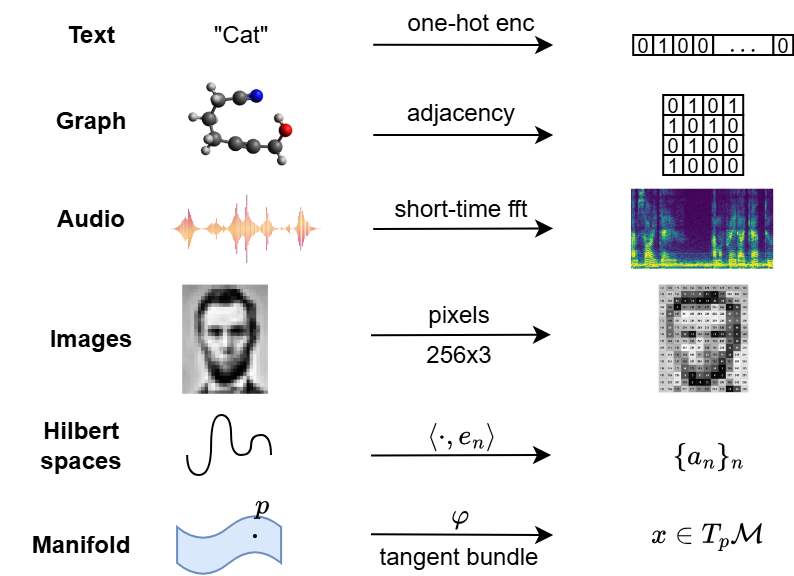
\includegraphics[width=\textwidth]{representation_examples.png}
\end{column}
\begin{column}{0.52\textwidth}
\footnotesize
Words, molecules, sounds and images are not vectors, and every model of this course takes its input in $\R^d$. A map $\varphi:\{\text{objects}\}\to\R^d$ comes first: the \alert{representation}.
\begin{itemize}
\item It is a \alert{modelling choice}: it decides which information the model receives, and in which geometry.
\item Lecture 02 made it without saying so: a digit was its $784$ grey levels.
\item $\varphi$ can be \alert{designed} from what is known about the objects, or \alert{learned} with the model.
\end{itemize}
\end{column}
\end{columns}
\nbref{09 \S3}
\end{frame}


% =========================================================================
\begin{frame}{Text for a language model: tokens, embeddings, positions}
\begin{columns}[c]
\begin{column}{0.51\textwidth}
\centering
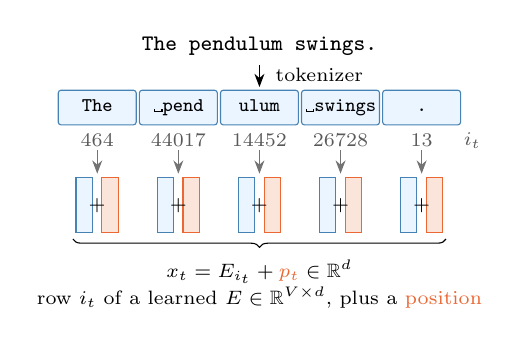
\begin{tikzpicture}[x=1.03cm, y=1cm, >=Stealth, font=\scriptsize,
    tokbox/.style={draw=boxframe, fill=boxbg, rounded corners=1pt, minimum height=4.4mm, minimum width=9.9mm,
                   inner sep=1.2pt, font=\ttfamily\scriptsize},
    embvec/.style={draw=boxframe, fill=boxbg, minimum width=2.1mm, minimum height=7mm, inner sep=0pt},
    posvec/.style={draw=ctrl, fill=ctrl!18, minimum width=2.1mm, minimum height=7mm, inner sep=0pt}]
  \node[font=\ttfamily\footnotesize] (text) at (2,0) {The pendulum swings.};
  \draw[->] (text) -- (2,-0.52);
  \node[anchor=west] at (2.08,-0.36) {\alert{tokenizer}};
  \foreach \i/\t/\id in {0/The/464, 1/\textvisiblespace pend/44017, 2/ulum/14452, 3/\textvisiblespace swings/26728, 4/./13} {
    \node[tokbox] (t\i) at (\i,-0.78) {\strut\t};
    \node[text=black!65, inner sep=1pt] (i\i) at (\i,-1.2) {\id};
    \draw[->, black!55] (i\i) -- (\i,-1.62);
    \node[embvec] at (\i-0.16,-2.02) {};
    \node[posvec] at (\i+0.16,-2.02) {};
    \node at (\i,-2.02) {$+$};
  }
  \node[anchor=west, text=black!65, inner sep=1pt] at (4.48,-1.2) {$i_t$};
  \draw[decorate, decoration={brace, mirror, amplitude=3pt}] (-0.3,-2.45) -- (4.3,-2.45);
  \node[align=center] at (2,-3.02) {$x_t=E_{i_t}+\ctrl{p_t}\in\R^d$\\ row $i_t$ of a learned $E\in\R^{V\times d}$, plus a \ctrl{position}};
\end{tikzpicture}
\end{column}
\begin{column}{0.485\textwidth}
\centering
\scriptsize
\renewcommand{\arraystretch}{1.15}
\setlength{\tabcolsep}{2.5pt}
\begin{tabular}{@{}l r r r@{}}
\toprule
 & $V$ & $d$ & context \\
\midrule
Transformer & $\approx37\,000$ & $512$ & \\
GPT-2 & $50\,257$ & $768$--$1600$ & $1024$ \\
GPT-3 & $50\,257$ & $12\,288$ & $2048$ \\
Llama 3 & $128\,000$ & $4096$--$16\,384$ & $128$K \\
\bottomrule
\end{tabular}

\smallskip
\raggedright
$V$ tokens in the vocabulary, vectors of dimension $d$, longest input in tokens \citep{vaswani2017,radford2019,brown2020,grattafiori2024}.
\end{column}
\end{columns}

\smallskip
\footnotesize
\begin{itemize}
\item A \alert{token} is a piece of a word, not a word: \texttt{pendulum} is two tokens. The tokenizer is fixed before training \citep{sennrich2016}; this one is the tokenizer of GPT-2.
\item $E$ is \alert{learned}: a linear layer on one-hot vectors. In GPT-3 it has $Vd=6.2\cdot10^{8}$ entries, and a full context is $2048\times12\,288=2.5\cdot10^{7}$ numbers.
\item \ctrl{Positions} \citep{vaswani2017}: $p_t=\big(\sin(\omega_jt),\cos(\omega_jt)\big)_{j<d/2}$ with $\omega_j=10000^{-2j/d}$, sines and cosines of $t$ at $d/2$ frequencies. A learned table of positions gives nearly identical results. Without $p_t$ the model would not see the \alert{order} of the words: part 2.
\end{itemize}
\nbref{15 \S4}
\end{frame}


% =========================================================================
\begin{frame}{A change of coordinates changes the problem}
\begin{columns}[T]
\begin{column}{0.45\textwidth}
\footnotesize
\alert{Two rings.} One linear classifier, in two coordinate systems.

\smallskip
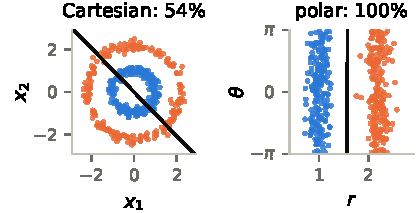
\includegraphics[width=\textwidth]{rings_coordinates.pdf}

\smallskip
In $(x_1,x_2)$ no line separates the rings: $54\%$ of the points are classified correctly. In $\varphi(x)=(r,\theta)$ one does: $100\%$.
\end{column}
\begin{column}{0.5\textwidth}
\footnotesize
\alert{The digits.} An affine change is enough. The baseline of lecture 02, on the same $784$ numbers:

\medskip
{\centering
\renewcommand{\arraystretch}{1.2}
\begin{tabular}{@{}l r r@{}}
\toprule
\textbf{Input} & \textbf{1 epoch} & \textbf{5 epochs} \\
\midrule
bytes in $[0,255]$ & $89.5\%$ & $92.7\%$ \\
grey levels in $[0,1]$ & $91.2\%$ & $94.3\%$ \\
centred, $x-\bar x$ & $93.0\%$ & $95.2\%$ \\
\bottomrule
\end{tabular}
\par}

\medskip
{\scriptsize Test accuracy, mean of three initializations; $\bar x$ is the mean image. The run of lecture 02, with $94.0\%$, is one of the second row.\par}
\end{column}
\end{columns}

\smallskip
\footnotesize
\alert{A reason.} For a linear model $w\cdot x$ and the squared loss, $\nabla^2F=\frac1N\sum_ix_ix_i^\top=C+\bar x\,\bar x^\top$, with $C$ the covariance of the inputs. The mean image adds an eigenvalue of size $|\bar x|^2=35$ to those of $C$, which are at most $5.1$: $L=38$. Centring divides $L$ by $7.4$, and bytes multiply it by $255^2$. In lecture 02, $L$ limited the step size. A network trained with Adam is not this model: the effect is smaller, and still there.
\end{frame}


% =========================================================================
\begin{frame}{Fourier features: only the input changes}
\footnotesize
Target $g(x)+0.3\sin(20x)$; $\tanh$ network, two hidden layers of 64 neurons; squared error; Adam, $\eta=10^{-3}$. Input: $x$, or its first $m$ harmonics $\varphi_m(x)=\big(\cos(j\pi x/2),\,\sin(j\pi x/2)\big)_{j\le m}\in\R^{2m}$.

\smallskip
\centerline{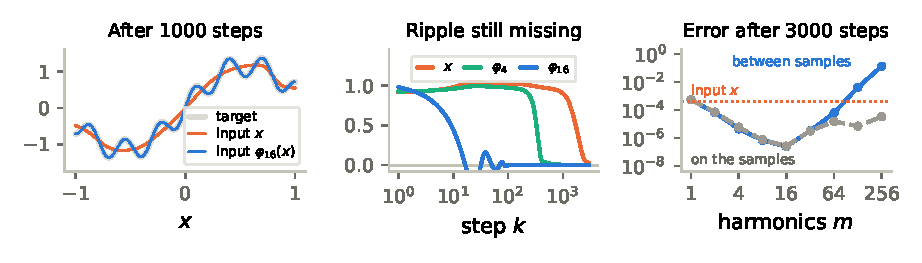
\includegraphics[width=0.86\textwidth]{fourier_features.pdf}}

\begin{itemize}
\item \alert{The ripple is fitted}, with less than $10\%$ missing, from step $2350$ with $x$ and from step $44$ with $\varphi_{16}(x)$. Five initializations: $30$ to $44$, against $1955$ to over $3000$.
\item \alert{The price:} 32 inputs for one, and a scale to choose: $m=1$ gains nothing, and $m=256$ fits the 160 samples but is wrong between them (error $0.13$). And $\varphi$ must stay injective: with period 2, $\varphi(-1)=\varphi(1)$ and the error stays at $6.4\cdot10^{-3}$.
\item This map is the positional encoding of the previous frame \citep{tancik2020}. Why the plain network is slow: part 5.
\end{itemize}
\end{frame}


% =========================================================================
\begin{frame}{How large is what the model sees?}
\scriptsize
\renewcommand{\arraystretch}{1.2}
\begin{tabularx}{\textwidth}{@{}>{\raggedright\arraybackslash}p{0.17\textwidth} >{\raggedright\arraybackslash}X >{\raggedleft\arraybackslash}p{0.245\textwidth}@{}}
\toprule
\textbf{Input of} & \textbf{What it receives} & \textbf{Numbers} \\
\midrule
vision transformer \citep{dosovitskiy2021} & $224\times224\times3$ pixels, cut into $196$ patches of $16\times16$; each patch is mapped linearly to $\R^{768}$: a token & $150\,528\to196\times768$ \\
latent diffusion \citep{rombach2022} & $256\times256\times3$ pixels, which an autoencoder turns into a latent of shape $32\times32\times4$ & $196\,608\to4\,096$ \\
the baseline & a digit as its $784$ grey levels, or as its first $k$ \alert{principal components} & $784\to k$ \\
\bottomrule
\end{tabularx}

\smallskip
\centerline{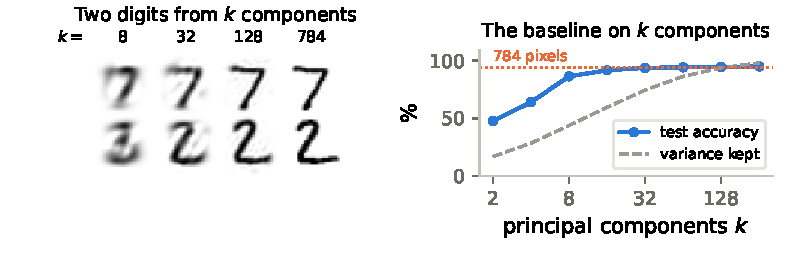
\includegraphics[width=0.7\textwidth]{mnist_pca.pdf}}

\footnotesize
\alert{Principal components:} the coordinates of an image along the $k$ orthogonal directions of largest variance. With only its input changed, the baseline reaches $94.05\%$ on $64$ components ($86\%$ of the variance), against $94.00\%$ on the $784$ pixels: $1\,482$ parameters instead of $13\,002$.
\end{frame}


% =========================================================================
\begin{frame}{Designed or learned?}
\vspace{1.5mm}
\centerline{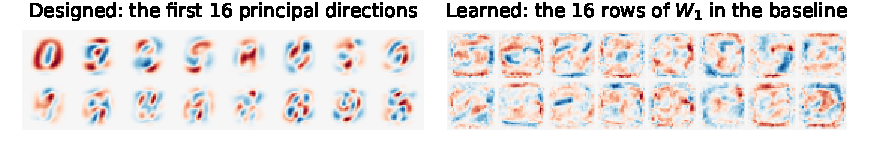
\includegraphics[width=0.95\textwidth]{mnist_directions.pdf}}

\footnotesize
The network of lecture 02 is a \alert{linear} classifier on a \alert{learned} representation $\psi$:
\[
f(x;w)=W_3\,\psi(x)+b_3,\qquad\psi(x)=\sigma\big(W_2\,\sigma(W_1x+b_1)+b_2\big)\in\R^{16}.
\]
The same linear classifier on 16 numbers reaches $84.9\%$ on 16 principal components and $94.0\%$ on the 16 learned features $\psi(x)$. On all $784$ pixels it reaches $92.5\%$.

\smallskip
\renewcommand{\arraystretch}{1.2}
\begin{tabularx}{\textwidth}{@{}>{\raggedright\arraybackslash}X >{\raggedright\arraybackslash}X@{}}
\toprule
\textbf{Designed:} $(\cos q,\sin q)$ for an angle, $(q,\dot q)$ for an oscillation, Fourier features, spectrograms, principal components & \textbf{Learned:} the embedding matrix $E$, the projection of the patches, the hidden layers of a network \\
\midrule
knowledge enters before training; little or nothing to fit; the same for every task & found by the optimizer; needs data; adapted to the task; hard to read \\
\bottomrule
\end{tabularx}

\smallskip
\alert{Which representations can be learned is decided by the next box: the architecture.}
\end{frame}


% #########################################################################
% PART 2: ARCHITECTURE
% #########################################################################

% Part 2: architecture.  Figures and numbers: figures/part2_depth.py and figures/part2_mnist.py.

% =========================================================================
\section{Architecture}

\begin{frame}{An architecture is a structure built into the family}
\centering
\loopdiagram{2}

\smallskip
\footnotesize
\renewcommand{\arraystretch}{1.12}
\begin{tabularx}{\textwidth}{@{}l l >{\raggedright\arraybackslash}X@{}}
\toprule
 & \textbf{One layer} & \textbf{Symmetry; dynamical reading} \\
\midrule
\alert{MLP} & $x_{k+1}=\sigma(W_kx_k+b_k)$ & none; layers are time steps \\
\alert{CNN} & $x_{k+1}=\sigma(K_k\star x_k+b_k)$ & translations of a grid; a finite-difference stencil \\
\alert{RNN} & $h_{t}=\sigma(W_hh_{t-1}+W_x\ctrl{x_t}+b)$ & translations in time; a system driven by the input $\ctrl{x_t}$ \\
\alert{ResNet} & $x_{k+1}=x_k+h\,\sigma(\ctrl{W_k}x_k+\ctrl{b_k})$ & none; an Euler scheme whose control is the weights \\
\alert{Transformer} & $x_i\leftarrow x_i+\sum_ja_{ij}(x)\,Vx_j$ & permutations of the tokens; interacting particles \\
\bottomrule
\end{tabularx}

\smallskip
\raggedright
Data, loss and optimizer stay the same; the family $\{f(\,\cdot\,;w)\}$ changes. \alert{Choosing an architecture is choosing what to assume} \citep{bronstein2021}.
\nbref{09 \S14, 13, 15}
\end{frame}


% =========================================================================
\begin{frame}[fragile]{Three layers for one input, and what they assume}
\footnotesize
\begin{columns}[c]
\begin{column}{0.41\textwidth}
\alert{MLP} \citep{rumelhart1986}. \ $x\mapsto\sigma(Wx+b)$.

\smallskip
\alert{Nothing assumed:} relabelling the inputs, $x\mapsto\Pi x$, only replaces $W$ by $W\Pi^\top$. The family does not know which pixels are neighbours.
\end{column}
\begin{column}{0.59\textwidth}
\begin{lstlisting}
x = torch.randn(784)       # flattened image
layer = nn.Linear(784, 16) # 12560 parameters
y = torch.relu(layer(x))   # shape (16,)
\end{lstlisting}
\end{column}
\end{columns}

\medskip
\begin{columns}[c]
\begin{column}{0.41\textwidth}
\alert{CNN} \citep{lecun1998}. \ $x\mapsto\sigma(K\star x+b)$.

\smallskip
\alert{Translation equivariance:} $K\star(Tx)=T(K\star x)$ for a shift $T$ of a periodic grid. Eight $5\times5$ kernels have $208$ parameters, for an image of any size.
\end{column}
\begin{column}{0.59\textwidth}
\begin{lstlisting}
x = torch.randn(1, 28, 28)   # 1 channel
conv = nn.Conv2d(1, 8, 5, padding=2,
                 padding_mode="circular")
T = lambda x: x.roll((3, 5), (1, 2)) # shift
torch.allclose(conv(T(x)), T(conv(x)),
               atol=1e-6)    # True
\end{lstlisting}
\end{column}
\end{columns}

\medskip
\begin{columns}[c]
\begin{column}{0.41\textwidth}
\alert{ResNet} \citep{he2016}. \ $x\mapsto x+h\,\sigma(Wx+b)$.

\smallskip
\alert{Close to the identity:} $\|f(x)-x\|\le h\sqrt d$ if $|\sigma|\le1$. An Euler step of $\dot x=\sigma(Wx+b)$, as in lecture 01.
\end{column}
\begin{column}{0.59\textwidth}
\begin{lstlisting}
x, h = torch.randn(16), 0.1
layer = nn.Linear(16, 16)
y = x + h * torch.tanh(layer(x)) # one step
(y - x).norm() <= h * 16 ** 0.5  # True
\end{lstlisting}
\end{column}
\end{columns}
\nbref{09 \S14, 13}
\end{frame}


% =========================================================================
\begin{frame}[fragile]{Two layers for sequences, and what they assume}
\footnotesize
\begin{columns}[c]
\begin{column}{0.41\textwidth}
\alert{RNN} \citep{elman1990}. \ $h_t=\sigma(W_hh_{t-1}+W_xx_t+b)$.

\smallskip
\alert{Time invariance:} the same weights at every step, for any length. Restarting from $h_s$ reproduces $h_{s+1},h_{s+2},\dots$
\end{column}
\begin{column}{0.59\textwidth}
\begin{lstlisting}
x = torch.randn(20, 3)       # 20 steps in R^3
rnn = nn.RNN(3, 8)           # 104 parameters
h, _ = rnn(x)                # shape (20, 8)
tail, _ = rnn(x[5:], h[4:5]) # restart at h_5
torch.allclose(tail, h[5:], atol=1e-6) # True
\end{lstlisting}
\end{column}
\end{columns}

\smallskip
\alert{Transformer} \citep{vaswani2017}. Tokens: the rows of $X\in\R^{T\times d}$. One head of attention:
\[
\mathrm{Attn}(X)=\softmax(A)\,XW_V,\quad A=XW_Q\,(XW_K)^{\!\top}/\sqrt d,\quad\text{softmax along each row.}
\]
\vspace{-0.6\baselineskip}
\begin{columns}[c]
\begin{column}{0.41\textwidth}
\alert{Permutation equivariance:} $\mathrm{Attn}(\Pi X)=\Pi\,\mathrm{Attn}(X)$ for every permutation matrix $\Pi$, since $\softmax(\Pi A\Pi^\top)=\Pi\softmax(A)\Pi^\top$.
\end{column}
\begin{column}{0.59\textwidth}
\begin{lstlisting}
x = torch.randn(10, 32)      # 10 tokens in R^32
attn = nn.MultiheadAttention(32, 4) # 4 heads
y, _ = attn(x, x, x)         # shape (10, 32)
p = torch.randperm(10)       # a permutation
z, _ = attn(x[p], x[p], x[p])
torch.allclose(z, y[p], atol=1e-6)  # True
\end{lstlisting}
\end{column}
\end{columns}

\smallskip
Attention ignores the order of the tokens: hence the \alert{positional encoding} of part 1.
\nbref{09 \S14, 15}
\end{frame}


% =========================================================================
\begin{frame}{Convolution: the symmetry decides the architecture}
\small
On a periodic grid, $x\in\R^n$: shift $(Tx)_i=x_{i-1}$, convolution $(k\star x)_i=\sum_jk_j\,x_{i-j}$.
\begin{mathbox}{Proposition (translation equivariance)}
A linear map $A:\R^n\to\R^n$ commutes with the shift, $AT=TA$, if and only if it is a convolution: $Ax=k\star x$ for some kernel $k\in\R^n$.
\end{mathbox}
\footnotesize
\emph{Proof of ``only if''.} Let $k=A\,\delta_0$, the response to a unit impulse. Since $x=\sum_jx_j\,T^j\delta_0$,
\[
Ax=\sum_jx_j\,T^jA\,\delta_0=\sum_jx_j\,T^jk=k\star x. \qquad\square
\]
\begin{columns}[c]
\begin{column}{0.60\textwidth}
\begin{itemize}
\item \alert{Weight sharing.} A dense layer on a $28\times28$ image has $784^2=614\,656$ weights, a $3\times3$ convolution $9$.
\item \alert{A stencil.} With $k=(1,-2,1)/h^2$, $x+\tau\,k\star x$ is an explicit Euler step of the heat equation $y_t=y_{xx}$.
\end{itemize}
\end{column}
\begin{column}{0.40\textwidth}
\centering
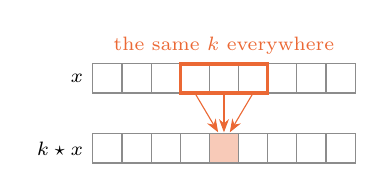
\begin{tikzpicture}[x=3.7mm, y=3.7mm, >=Stealth, font=\scriptsize]
  \foreach \i in {0,...,8} \draw[black!45] (\i,2.4) rectangle ++(1,1);
  \foreach \i in {0,...,8} \draw[black!45] (\i,0) rectangle ++(1,1);
  \draw[ctrl, very thick] (3,2.4) rectangle (6,3.4);
  \fill[ctrl!35] (4,0) rectangle (5,1);
  \draw[black!45] (4,0) rectangle (5,1);
  \draw[->, ctrl] (3.5,2.4) -- (4.3,1.05);
  \draw[->, ctrl] (4.5,2.4) -- (4.5,1.05);
  \draw[->, ctrl] (5.5,2.4) -- (4.7,1.05);
  \node[left] at (0,2.9) {$x$};
  \node[left] at (0,0.5) {$k\star x$};
  \node[above, ctrl] at (4.5,3.4) {the same $k$ everywhere};
\end{tikzpicture}
\end{column}
\end{columns}
\nbref{09 \S14.2}
\end{frame}


% =========================================================================
\begin{frame}{What depth buys: the parity of $n$ bits}
\footnotesize
\alert{Parity:} $x_1\oplus\dots\oplus x_n=1$ when the number of ones is odd; with bits $\pm1$, the product $x_1x_2\cdots x_n$. Classical: one threshold neuron cannot compute it, even for $n=2$ \citep{minsky1969}.

\centering
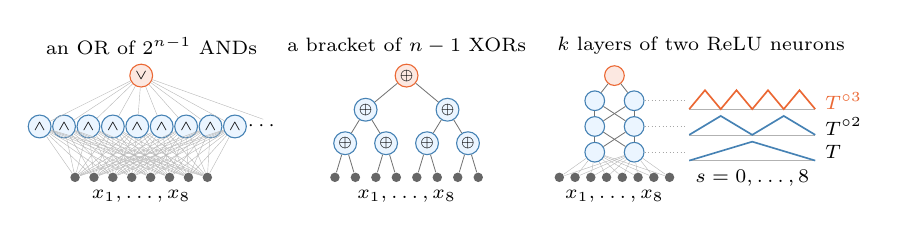
\begin{tikzpicture}[x=1cm, y=0.76cm, font=\scriptsize,
    bit/.style={circle, fill=black!60, inner sep=0pt, minimum size=1.2mm},
    gate/.style={circle, draw=boxframe, fill=boxbg, inner sep=0pt, minimum size=2.9mm, font=\tiny},
    top/.style={draw=ctrl, fill=ctrl!15},
    wire/.style={black!28, line width=0.15pt},
    link/.style={black!55, line width=0.3pt}]
  % --- shallow and wide: an OR of 2^(n-1) ANDs, each reading all n bits (drawn for n = 8) ---
  \foreach \i in {0,...,7} \node[bit] (a\i) at ({0.45+0.24*\i},0) {};
  \foreach \j in {0,...,8} \node[gate] (and\j) at ({0.31*\j},0.85) {$\wedge$};
  \node at (2.84,0.85) {$\cdots$};
  \node[gate, top] (or) at (1.29,1.7) {$\vee$};
  \foreach \i in {0,...,7} \foreach \j in {0,...,8} \draw[wire] (a\i) -- (and\j);
  \foreach \j in {0,...,8} \draw[wire] (and\j) -- (or);
  \draw[wire] (2.84,0.97) -- (or);
  \node[below] at (1.29,-0.05) {$x_1,\dots,x_8$};
  \node at (1.42,2.2) {an OR of $2^{n-1}$ ANDs};
  % --- deep and narrow: a tournament bracket of 2-input XORs ---
  \foreach \i in {0,...,7} \node[bit] (b\i) at ({3.75+0.26*\i},0) {};
  \foreach \j in {0,...,3} \node[gate] (p\j) at ({3.88+0.52*\j},0.57) {$\oplus$};
  \foreach \j in {0,1} \node[gate] (q\j) at ({4.14+1.04*\j},1.13) {$\oplus$};
  \node[gate, top] (r) at (4.66,1.7) {$\oplus$};
  \foreach \i/\j in {0/0,1/0,2/1,3/1,4/2,5/2,6/3,7/3} \draw[link] (b\i) -- (p\j);
  \foreach \i/\j in {0/0,1/0,2/1,3/1} \draw[link] (p\i) -- (q\j);
  \foreach \i in {0,1} \draw[link] (q\i) -- (r);
  \node[below] at (4.66,-0.05) {$x_1,\dots,x_8$};
  \node at (4.66,2.2) {a bracket of $n-1$ XORs};
  % --- k layers of two ReLU neurons: the hat function composed k times ---
  \foreach \i in {0,...,7} \node[bit] (c\i) at ({6.6+0.2*\i},0) {};
  \foreach \l/\y in {1/0.42,2/0.85,3/1.28} {
    \node[gate, minimum size=2.5mm] (u\l) at (7.05,\y) {};
    \node[gate, minimum size=2.5mm] (v\l) at (7.55,\y) {};
  }
  \node[gate, top, minimum size=2.5mm] (o) at (7.3,1.7) {};
  \foreach \i in {0,...,7} { \draw[wire] (c\i) -- (u1); \draw[wire] (c\i) -- (v1); }
  \foreach \l/\m in {1/2,2/3} {
    \draw[link] (u\l) -- (u\m); \draw[link] (u\l) -- (v\m);
    \draw[link] (v\l) -- (u\m); \draw[link] (v\l) -- (v\m);
  }
  \draw[link] (u3) -- (o); \draw[link] (v3) -- (o);
  \node[below] at (7.3,-0.05) {$x_1,\dots,x_8$};
  % what the network has computed after each layer, as a function of the number of ones s
  \foreach \l/\y in {1/0.42,2/0.85,3/1.28} \draw[black!35, densely dotted, line width=0.3pt] (v\l) -- (8.2,\y);
  \begin{scope}[shift={(8.25,0.28)}, x=0.2cm, y=0.24cm]
    \draw[black!30, line width=0.2pt] (0,0) -- (8,0);
    \draw[boxframe, line width=0.6pt] (0,0) -- (4,1) -- (8,0);
  \end{scope}
  \begin{scope}[shift={(8.25,0.71)}, x=0.2cm, y=0.24cm]
    \draw[black!30, line width=0.2pt] (0,0) -- (8,0);
    \draw[boxframe, line width=0.6pt] (0,0) -- (2,1) -- (4,0) -- (6,1) -- (8,0);
  \end{scope}
  \begin{scope}[shift={(8.25,1.14)}, x=0.2cm, y=0.24cm]
    \draw[black!30, line width=0.2pt] (0,0) -- (8,0);
    \draw[ctrl, line width=0.6pt] (0,0) -- (1,1) -- (2,0) -- (3,1) -- (4,0) -- (5,1) -- (6,0) -- (7,1) -- (8,0);
  \end{scope}
  \node[right] at (9.85,0.42) {$T$};
  \node[right] at (9.85,0.85) {$T^{\circ2}$};
  \node[right, text=ctrl] at (9.85,1.28) {$T^{\circ3}$};
  \node[below] at (9.05,0.28) {$s=0,\dots,8$};
  \node at (8.4,2.2) {$k$ layers of two ReLU neurons};
\end{tikzpicture}

\raggedright
\scriptsize
\begin{columns}[T]
\begin{column}{0.48\textwidth}
\alert{Gates AND, OR, NOT.} In an OR of ANDs each AND contains all $n$ variables, since flipping a missing one changes the parity: it accepts one input, and $2^{n-1}$ are odd. At depth $d$: size $\ge\exp(c_d\,n^{1/(d-1)})$ \citep{hastad1986}, after \citep{furst1984,ajtai1983,yao1985}. $n=20$: $524\,288$ ANDs, $19$ XORs.
\end{column}
\begin{column}{0.52\textwidth}
\alert{Neurons add.} Parity depends on $s=x_1+\dots+x_n$ only: one layer of $n$ neurons $\mathbf 1[s\ge j]$, with signs $+,-,+,\dots$ \citep{rumelhart1986pdp}. In $s$ it is a \alert{sawtooth}: for $2^k\ge n$ it is $T^{\circ k}(s/2^k)$, $T(t)=2\sigma(t)-4\sigma(t-\tfrac12)$ \citep{telgarsky2015,telgarsky2016}. $n=20$: $20$ neurons, or $10$ in $5$ layers.
\end{column}
\end{columns}

\smallskip
\footnotesize
\begin{mathbox}{Theorem (Telgarsky, 2016): no shallow network comes close}
For every $k\ge1$ there is a ReLU network $f$ with $2k^3+8$ layers and $3k^3+12$ nodes such that $\int_{[0,1]^d}|f-g|\,dx\ge\tfrac1{64}$ for every ReLU network $g$ with at most $k$ layers and at most $2^k$ nodes.
\end{mathbox}
\end{frame}


% =========================================================================
\begin{frame}{Digits: depth against width}
\footnotesize
\begin{columns}[c]
\begin{column}{0.48\textwidth}
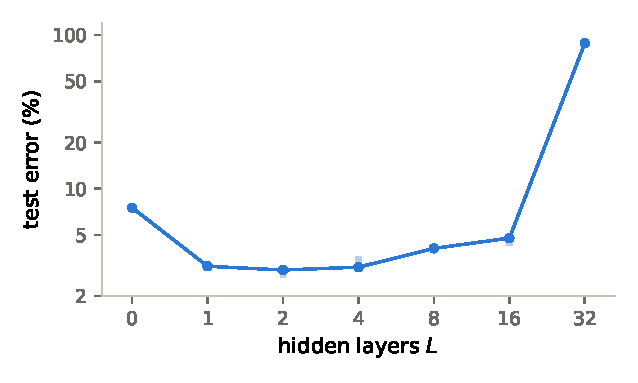
\includegraphics[width=\textwidth]{mnist_depth_width.pdf}
\end{column}
\begin{column}{0.52\textwidth}
\alert{Only the architecture box changes.} The data, the cross-entropy, Adam ($\eta=10^{-3}$, batches of 64, 5 epochs) and the seeds are those of the baseline $784\to16\to16\to10$, at $94.0\%$.

\medskip
\alert{Width helps.} With two hidden layers the test error falls from $7.6\%$ at width 8 to $2.2\%$ at width 128, with $118\,282$ parameters.
\end{column}
\end{columns}

\smallskip
\alert{Depth does not, here.} For widths from 16 on, the networks with 1, 2 and 4 hidden layers differ by at most $0.8$ points. Three initializations of the baseline give $93.6\%$, $94.0\%$ and $94.4\%$: a difference of the same size. At width 8, four layers are worse: $9.3\%$ against $7.6\%$. In the baseline the first layer, $784\times16$, holds $97\%$ of the parameters.

\smallskip
The theorems on depth say what \emph{can} be represented with few neurons. Here the number of layers is not the obstacle: these networks ignore that the input is an image.

\smallskip
\scriptsize Rates of approximation for fixed families and the curse of dimensionality: appendix.
\end{frame}


% =========================================================================
\begin{frame}[fragile]{Digits: a convolutional network}
\footnotesize
\begin{columns}[c]
\begin{column}{0.60\textwidth}
\begin{lstlisting}
cnn = nn.Sequential(
  nn.Unflatten(1, (1, 28, 28)),   # 1x28x28
  nn.Conv2d(1, 8, 5), nn.ReLU(),  # 8x24x24
  nn.MaxPool2d(2),                # 8x12x12
  nn.Conv2d(8, 16, 5), nn.ReLU(), # 16x8x8
  nn.MaxPool2d(2), nn.Flatten(),  # 256
  nn.Linear(256, 10))             # 10 scores
\end{lstlisting}
\begin{itemize}
\item A small LeNet \citep{lecun1998}; the same data, loss, optimizer and epochs. $5\,994$ parameters, fewer than half of the baseline's: test error \alert{$1.3\%$} instead of $6.0\%$.
\item $906$ parameters ($c=2$): $3.6\%$. The smallest fully connected network above that does as well has $50\,890$.
\item \alert{Shuffle the pixels} with one fixed permutation. The fully connected network does not notice: $5.8\%$, from $6.0\%$. The convolutional one falls to the same $5.8\%$.
\end{itemize}
\end{column}
\begin{column}{0.40\textwidth}
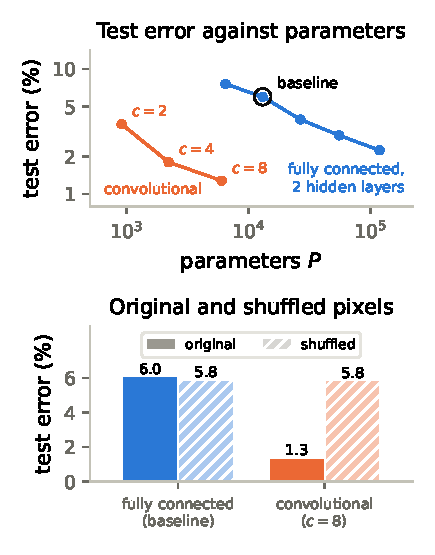
\includegraphics[width=\textwidth]{mnist_cnn.pdf}

\smallskip
\alert{An architecture is an assumption on the data.} When it fails, nothing is gained.
\end{column}
\end{columns}
\end{frame}


% #########################################################################
% PART 3: LOSS
% #########################################################################

% Part 3: Loss.  Figures and numbers: figures/part3_loss.py (see images/SOURCES_part3.md).

% =========================================================================
\section{Loss}

\begin{frame}{The loss states what an error is}
\centering
\loopdiagram{3}

\raggedright\footnotesize
\smallskip
The loss $\ell(\hat y,y)\ge0$ compares the output of the model with the label. \alert{Each problem has its own:}

\smallskip
\renewcommand{\arraystretch}{1.25}
\begin{tabularx}{\textwidth}{@{}l l >{\raggedright\arraybackslash}X@{}}
\toprule
\textbf{Problem} & \textbf{Output of the model} & \textbf{Loss} \\
\midrule
regression & a number $\hat y=f(x;w)$ & squared: $(\hat y-y)^2$ \\
regression with outliers & a number $\hat y$ & absolute: $|\hat y-y|$, or Huber \citep{huber1964} \\
classification, $K$ classes & probabilities $p_1,\dots,p_K$ & cross-entropy: $-\log p_y$ \\
one rare class & a probability $p$ & weighted cross-entropy \\
several possible answers & a law $p(\,\cdot\mid x;w)$ for $y$ & log-loss: $-\log p(y\mid x;w)$ \\
\bottomrule
\end{tabularx}

\medskip
Lecture 02 used the first row for the curve $g$ and the third for the digits. Three questions: where do these losses come from, what does each of them learn, and what changes when one class is rare?
\end{frame}


% =========================================================================
\begin{frame}{Maximum likelihood: one principle, many losses}
\footnotesize
Let the model output a \alert{law} $p(y\mid x;w)$ for the label, instead of one value. For independent samples, maximizing the likelihood $\prod_ip(y_i\mid x_i;w)$ is minimizing the empirical risk of the \alert{log-loss}:
\[
F(w)=-\frac1N\sum_{i=1}^N\log p(y_i\mid x_i;w),\qquad\ell=-\log p(y\mid x;w).
\]
\begin{mathbox}{Three models of the noise, three losses $-\log p(y\mid x;w)$}
\renewcommand{\arraystretch}{1.35}
\begin{tabularx}{\linewidth}{@{}>{\raggedright\arraybackslash}X l@{}}
Gaussian: \ $y=f(x;w)+\varepsilon$,\ \ $\varepsilon\sim\mathcal N(0,s^2)$ & $\tfrac1{2s^2}\,(y-f(x;w))^2+\text{const}$ \\
Laplace: \ $y=f(x;w)+\varepsilon$,\ \ $\varepsilon$ of density $\tfrac1{2b}\,e^{-|\varepsilon|/b}$ & $\tfrac1b\,|y-f(x;w)|+\text{const}$ \\
Categorical: \ $\Prob(y=j\mid x)=p_j(x;w)$ & $-\log p_y(x;w)$ \\
\end{tabularx}
\end{mathbox}
The squared loss, the absolute loss and the cross-entropy are one loss, for three models of the noise.

\smallskip
\alert{In expectation.} If $y$ is discrete, or has a conditional density $\rho(y\mid x)$ of finite entropy,
\[
\Risk(w)=\E_x\Big[\KL\big(\rho(\,\cdot\mid x)\,\big\|\,p(\,\cdot\mid x;w)\big)\Big]+H,\qquad H=\E\big[-\log\rho(y\mid x)\big].
\]
$H$ does not depend on $w$: maximum likelihood minimizes the Kullback--Leibler divergence from the data to the model.
\nbref{09 \S4}
\end{frame}


% =========================================================================
\begin{frame}{The loss decides what is learned}
\footnotesize
\begin{mathbox}[top=1pt, bottom=1pt]{Proposition (the minimizers of three population risks)}
Let $(x,y)\sim\rho$ with $y\in\R$ and $\E\,y^2<\infty$. Among all functions $f$ of $x$ and all conditional densities $q$ of $y$ given $x$:
\begin{enumerate}
\item $\E\,(f(x)-y)^2$ is minimal for $f(x)=\E[y\mid x]$, the \alert{conditional mean};
\item $\E\,|f(x)-y|$ is minimal for $f(x)$ a \alert{median} of the law of $y$ given $x$;
\item $\E\big[-\log q(y\mid x)\big]$ is minimal only for $q=\rho(\,\cdot\mid x)$, the \alert{conditional law} itself.
\end{enumerate}
\end{mathbox}
\emph{Proof.} Minimize for each $x$ separately, with $a=f(x)$. (1) $\E\big[(a-y)^2\mid x\big]=\big(a-\E[y\mid x]\big)^2+\Var(y\mid x)$. (2) $a\mapsto\E\big[|a-y|\mid x\big]$ is convex with slope $\Prob(y<a\mid x)-\Prob(y>a\mid x)$, which changes sign at a median. (3) By the previous slide the risk is $\E_x\KL\big(\rho\,\|\,q\big)+H$, and $\KL\ge0$ with equality only for equal laws. \hfill$\square$
\begin{itemize}
\item The squared loss learns one number for each $x$, at best the mean. The log-loss learns a law: mean, median and spread follow from it \citep[Section~1.5]{bishop2006}.
\item The log-loss is \alert{strictly proper} (item 3), as is the squared error on the probabilities \citep{gneiting2007}, which gives $93.6\%$ on the digits (cross-entropy: $94.0\%$).
\item The accuracy sees a law only through its most probable class: of the $600$ test errors of the digit classifier, $86$ are made with a probability above $0.9$.
\end{itemize}
\end{frame}


% =========================================================================
\begin{frame}{Why predict a law: an inverse problem}
\footnotesize
Invert the target of lecture 02: $y$ uniform on $[-1,1]$, $x=g(y)+0.05\,\xi$, $\xi\sim\mathcal N(0,1)$; predict $y$ from $x$. For $0.44<|x|<1.16$ two values of $y$ are compatible with $x$.
\begin{center}
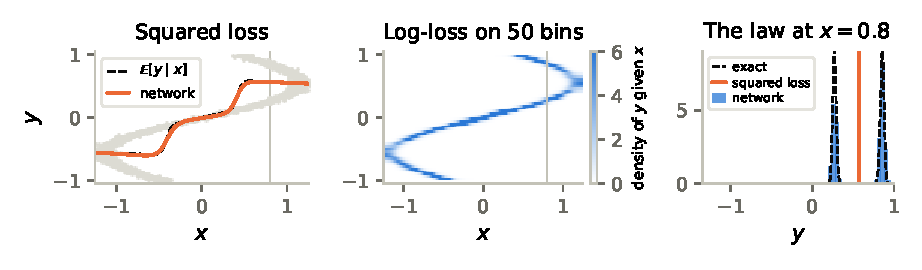
\includegraphics[width=0.80\textwidth]{inverse_problem_losses.pdf}
\end{center}
The same network twice ($1\to64\to64$, $\tanh$); only the output and the loss change.
\begin{itemize}
\item \alert{One output, squared loss.} The network finds $\E[y\mid x]$ (test RMSE $0.237$ for both). At $x=0.8$ it answers $0.57$, between the two solutions: $g(0.57)=1.16$.
\item \alert{50 bins of $y$, softmax and cross-entropy}, as for the digits. At $x=0.8$ the law has two bumps, at $0.26$ and $0.86$ (solutions: $0.268$ and $0.856$). Mean test log-density: $1.51$; exact law: $1.64$; a Gaussian around the squared-loss fit: $0.02$.
\item Language models output the law of the next token for the same reason \citep{vaswani2017}; inverse problems: \citep{bishop1994}.
\end{itemize}
\end{frame}


% =========================================================================
\begin{frame}{A rare event: accuracy says little}
\begin{columns}[T]
\begin{column}{0.66\textwidth}
\footnotesize
\alert{Anomaly detection.} $y=1$ for an anomaly: $1\%$ of the points. Normal points are $\mathcal N(0,I)$ in the plane, anomalies $\mathcal N(\mu,I)$ with $|\mu|=3$. A network $2\to16\to16\to1$ with the loss and the optimizer of the digits.

\medskip
$10^6$ test points, anomaly predicted when $p(x;w)>\tfrac12$:

\smallskip
{\centering
\renewcommand{\arraystretch}{1.15}
\begin{tabular}{@{}l r r@{}}
\toprule
 & \textbf{predicted anomaly} & \textbf{predicted normal} \\
\midrule
\textbf{anomaly} & $TP=5\,130$ & $FN=4\,744$ \\
\textbf{normal} & $FP=1\,497$ & $TN=988\,629$ \\
\bottomrule
\end{tabular}\par}
\end{column}
\begin{column}{0.30\textwidth}
\centering
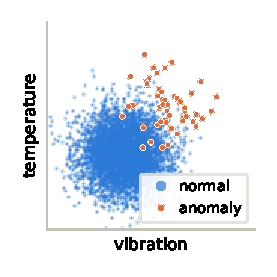
\includegraphics[width=\textwidth]{rare_event_data.pdf}

\scriptsize $5\,000$ training points,\\ 51 anomalies (orange)
\end{column}
\end{columns}

\footnotesize
\[
\begin{array}{@{}l@{\qquad}l@{}}
\text{accuracy}=\dfrac{TP+TN}{N}=99.38\%, & \text{\alert{precision}}=\dfrac{TP}{TP+FP}=0.77,\\[7pt]
\text{\alert{recall}}=\dfrac{TP}{TP+FN}=0.52, & \text{\alert{$F_1$}}=\dfrac{2\,TP}{2\,TP+FP+FN}=0.62 .
\end{array}
\]
\vspace{2pt}

Precision counts the alarms that are anomalies, recall the anomalies that are found; $F_1$ is their harmonic mean. The classifier that always answers ``normal'' has an accuracy of $99.01\%$, with recall $0$ and $F_1=0$: the accuracy is dominated by $TN$, which the other three leave out \citep{saito2015}.
\end{frame}


% =========================================================================
\begin{frame}{The threshold trades precision for recall}
\begin{center}
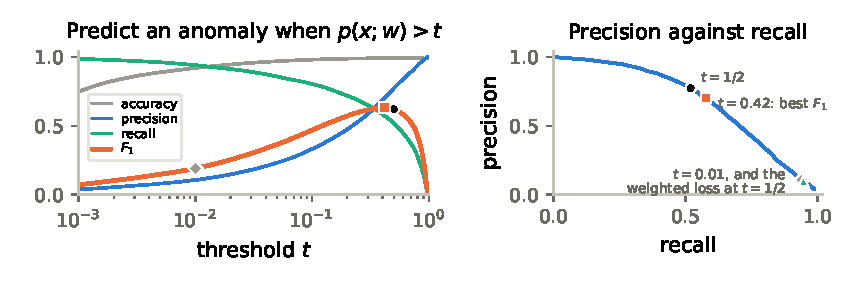
\includegraphics[width=0.93\textwidth]{rare_event_metrics.pdf}
\end{center}
\footnotesize
\begin{itemize}
\item \alert{The accuracy barely moves.} It is at least $99\%$ for every $t\ge0.22$, and largest, $99.38\%$, at $t=0.52$, where about half of the anomalies are missed.
\item \alert{A lower threshold} finds more anomalies and raises more false alarms. $F_1$ is largest at $t=0.42$ (chosen on validation data): precision $0.70$, recall $0.58$, $F_1=0.63$.
\item At $t=0.01$ the recall is $0.94$ and the precision $0.11$: nine alarms out of ten are false. The accuracy, $92.1\%$, is below that of the classifier that always answers ``normal''.
\end{itemize}
Which threshold is right depends on what a missed anomaly and a false alarm cost.
\end{frame}


% =========================================================================
\begin{frame}{Imbalance in the loss: a weight is a threshold}
\footnotesize
\begin{mathbox}{Proposition (weighted cross-entropy)}
Let $y\in\{0,1\}$, $p(x)=\Prob(y=1\mid x)$ and $c>0$. Among all functions $q$ of $x$ with values in $(0,1)$, the risk $\E\big[-c\,y\log q(x)-(1-y)\log(1-q(x))\big]$ is minimal for
\[
q^\star(x)=\frac{c\,p(x)}{c\,p(x)+1-p(x)},\qquad\text{so that}\qquad q^\star(x)>\tfrac12\iff p(x)>\frac1{1+c}.
\]
\end{mathbox}
\emph{Proof.} For each $x$ minimize $-c\,p\log q-(1-p)\log(1-q)$, convex in $q$: its derivative $-\frac{c\,p}{q}+\frac{1-p}{1-q}$ vanishes for $q\,(1-p)=c\,p\,(1-q)$. \hfill$\square$
\begin{itemize}
\item \alert{Weighting the loss is moving the threshold.} The weight $c$ is the cost of a missed anomaly, counted in false alarms \citep{elkan2001}. It adds $\log c$ to the score.
\item \alert{Experiment}, $c=99$: recall $0.95$, precision $0.10$, the triangle of the last figure. The plain network with $t=0.01$ decides the same on $98.9\%$ of the test points.
\item \alert{Relatives.} Repeating each anomaly $c$ times gives the same empirical risk. The focal loss $-(1-p_y)^\gamma\log p_y$ down-weights well-classified examples \citep{lin2017}.
\item \alert{The metric is not the loss.} Accuracy and $F_1$ are piecewise constant in $w$, with zero gradient almost everywhere. Train on the log-loss; choose $t$ on validation data.
\end{itemize}
\end{frame}


% #########################################################################
% PART 4: OPTIMIZATION
% #########################################################################

% Part 4: optimization.  Figures: figures/part4_sgd.py and figures/part4_mnist_batch.py.

% =========================================================================
\section{Optimization}

\begin{frame}{Optimization: which function do we minimize?}
\centering
\loopdiagram{4}

\smallskip
\raggedright\footnotesize
The samples $(x_i,y_i)$, $i=1,\dots,N$, are independent draws from an unknown law $\rho$. Data, architecture and loss being chosen, there are two functions of the parameters $w$:
\begin{mathbox}{Two risks}
\[
\underbrace{\Risk(w)=\E_{(x,y)\sim\rho}\,\ell\big(f(x;w),y\big)}_{\text{\alert{population risk}: what we want to be small}}
\qquad\quad
\underbrace{F(w)=\frac1N\sum_{i=1}^{N}\ell\big(f(x_i;w),y_i\big)}_{\text{\alert{empirical risk}: what we can evaluate}}
\]
\end{mathbox}
\begin{itemize}
\item $F$ is the population risk of the \alert{empirical measure} $\rho_N=\frac1N\sum_i\delta_{(x_i,y_i)}$: what is proved for a law $\rho$ also holds for $\rho_N$.
\item One gradient step on $F$ costs $N$ gradients. \alert{This part} samples the gradient: what is then minimized, what does the noise do, how does the batch size enter?
\end{itemize}
\nbref{09 \S2}
\end{frame}


% =========================================================================
\begin{frame}{Sampling the data is stochastic gradient descent}
\footnotesize
For a sample $z=(x,y)$ write $\ell_w(z)=\ell\big(f(x;w),y\big)$. A \alert{mini-batch gradient} averages $B$ independent draws $z_b\sim\rho$:
$g(w)=\frac1B\sum_{b=1}^{B}\nabla_w\ell_w(z_b)$.
\begin{mathbox}{Proposition (the sampled gradient is unbiased)}
Let $w'\mapsto\ell_{w'}(z)$ be Lipschitz near $w$ with a constant $G(z)$, $\E\,G(z)^2<\infty$, and differentiable at $w$ for $\rho$-almost every $z$. Then $\Risk$ is differentiable at $w$ and
\[
\E\,g(w)=\nabla\Risk(w),\qquad \Cov g(w)=\frac1B\,\Sigma(w),\qquad \Sigma(w)=\Cov_{z\sim\rho}\big(\nabla_w\ell_w(z)\big).
\]
\end{mathbox}
\emph{Proof.} $\big(\ell_{w+h}(z)-\ell_w(z)-\nabla_w\ell_w(z)\cdot h\big)/\|h\|\to0$ as $h\to0$ for almost every $z$, and is bounded by $2\,G(z)$: by dominated convergence $\nabla\Risk(w)=\E\,\nabla_w\ell_w(z)$. Covariances of independent gradients add. \hfill$\square$
\begin{itemize}
\item \alert{Fresh samples:} $\E[g_k\mid w_k]=\nabla\Risk(w_k)$. SGD is a stochastic approximation \citep{robbins1951}, a noisy Euler scheme for the gradient flow of the \alert{population} risk.
\item \alert{A fixed training set}, indices drawn with replacement: the proposition for $\rho_N$ gives $\E[g_k\mid w_k]=\nabla F(w_k)$. Once samples are reused, SGD descends $F$ and not $\Risk$.
\item \alert{Reshuffled epochs} (lecture 02): for a fixed $w$ a batch is unbiased, with covariance $\frac{N-B}{N-1}\,\frac{\Sigma}{B}$, zero for $B=N$; the batches of one epoch are dependent.
\end{itemize}
\end{frame}


% =========================================================================
\begin{frame}{Mini-batch SGD is an Euler--Maruyama scheme}
\footnotesize
Split the gradient into its mean and a centred noise, $g_k=\nabla F(w_k)+\zeta_k$. Then
\[
w_{k+1}=w_k-\eta\,\nabla F(w_k)-\sqrt\eta\,\big(\sqrt\eta\,\zeta_k\big),\qquad \Cov\big[\sqrt\eta\,\zeta_k\mid w_k\big]=\frac{\eta}{B}\,\Sigma(w_k).
\]
\begin{mathbox}{The stochastic modified equation \citep{li2017}}
\[
dW_t=-\nabla F(W_t)\,dt+\Big(\frac{\eta}{B}\,\Sigma(W_t)\Big)^{1/2}d\beta_t,\qquad t=k\eta,\quad\beta_t\text{ a Brownian motion}.
\]
SGD is its Euler--Maruyama scheme of step $\eta$, with $\sqrt\eta\,\zeta_k$ in the place of a Gaussian of the same covariance.
\end{mathbox}
\alert{Theorem \citep{li2017}.} For smooth losses, every $T>0$ and every $\psi$ of polynomial growth, $\big|\E\,\psi(w_k)-\E\,\psi(W_{k\eta})\big|\le C_{T,\psi}\,\eta$ for all $k\le T/\eta$: a \alert{weak approximation of order 1}.
\begin{itemize}
\item Lecture 02 added a noise $\sigma\sqrt\eta\,\xi_k$ with a fixed $\sigma$. Mini-batches give $\sigma^2=\frac{\eta}{B}\,\Sigma$: step and batch size enter the noise through the \alert{ratio $\eta/B$}, the temperature.
\item \alert{Weak:} laws, not paths, up to a finite time $T$. The noise of SGD is not Gaussian, and $\Sigma$ depends on $w$: no Gibbs measure $e^{-2F/\sigma^2}$ in general.
\item The equation contains $\eta$. As $\eta\to0$ the noise disappears and the gradient flow $\dot w=-\nabla F(w)$ remains.
\end{itemize}
\end{frame}


% =========================================================================
\begin{frame}{Near a minimum: an Ornstein--Uhlenbeck process}
\footnotesize
Near a minimizer: $F(w)\approx F^\star+\tfrac12(w-w^\star)^\top H\,(w-w^\star)$, and freeze $D=\frac{\eta}{B}\,\Sigma(w^\star)$.
\begin{mathbox}{A linear equation with the Gaussian stationary law $\mathcal N(w^\star,S)$}
\[
dW_t=-H\,(W_t-w^\star)\,dt+D^{1/2}d\beta_t,\quad\;
HS+SH=D,\quad\;
\E\,F(W)-F^\star=\frac{\eta}{4B}\operatorname{tr}\Sigma .
\]
\end{mathbox}
$S$ is the \alert{Gramian} $\Gram_\infty$ of lecture 01 for $\dot x=-Hx+D^{1/2}u$: white noise as the control.
\begin{center}
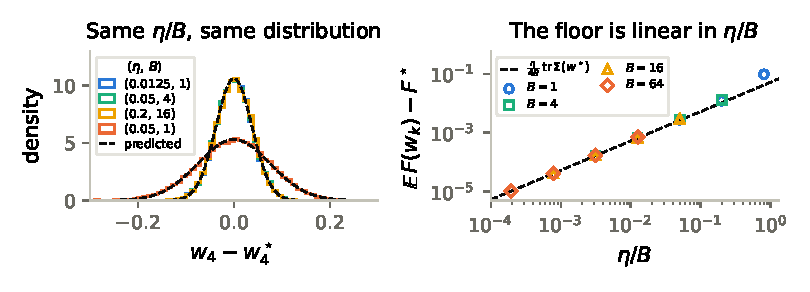
\includegraphics[width=0.71\textwidth]{sgd_stationary.pdf}
\end{center}
\scriptsize
Least squares with 8 hat functions on 160 noisy samples of $g$; 400 runs of SGD from $w^\star$. \alert{Left:} three pairs with $\eta/B=0.0125$ coincide with the prediction (dashed); $\eta/B=0.05$ doubles the spread. \alert{Right:} the floor is $\frac{\eta}{4B}\operatorname{tr}\Sigma$ within $5\%$ for $\eta\le0.05$. For $\eta=0.8$ it is higher: by $9\%$ because the step is not small, and by a factor $2.3$ for $B=1$, where $\Sigma(w)$ is far from constant.
\end{frame}


% =========================================================================
\begin{frame}{SGD with a constant step: the noise floor}
\footnotesize
\begin{mathbox}{Theorem (stochastic gradient descent with a constant step)}
Let $F$ be $L$-smooth with $\|\nabla F(w)\|^2\ge2\mu\big(F(w)-F^\star\big)$, as for a $\mu$-strongly convex $F$. Let $w_{k+1}=w_k-\eta\,g_k$, where $g_k$ is unbiased with bounded variance:
\[
\E\big[g_k\mid w_k\big]=\nabla F(w_k),\qquad\E\big[\|g_k-\nabla F(w_k)\|^2\mid w_k\big]\le\sigma^2 .
\]
Then, for $0<\eta\le1/L$,
\[
\E\,F(w_k)-F^\star\;\le\;(1-\eta\mu)^k\big(F(w_0)-F^\star\big)\;+\;\frac{\eta\,L\,\sigma^2}{2\mu}.
\]
\end{mathbox}
\emph{Proof.} Apply the descent lemma of lecture 02 with $v=w_k-\eta g_k$ and take the expectation given $w_k$, using $\E\|g_k\|^2\le\|\nabla F(w_k)\|^2+\sigma^2$ and then $1-L\eta/2\ge1/2$. With $\Delta_k=F(w_k)-F^\star$,
\[
\E\big[\Delta_{k+1}\mid w_k\big]\le\Delta_k-\tfrac\eta2\,\|\nabla F(w_k)\|^2+\tfrac12L\eta^2\sigma^2
\le(1-\eta\mu)\,\Delta_k+\tfrac12L\eta^2\sigma^2.
\]
Take expectations and iterate: $\E\Delta_k\le(1-\eta\mu)^k\Delta_0+\tfrac12L\eta^2\sigma^2\sum_{j<k}(1-\eta\mu)^j$, and the geometric sum is at most $1/(\eta\mu)$. \hfill$\square$

The first term is the rate of gradient descent, the second a \alert{floor proportional to $\eta\,\sigma^2$}. A batch of size $B$ has $\sigma^2=\operatorname{tr}\Sigma/B$ \citep{bottou2018}: the ratio $\eta/B$ again, as a bound.
\end{frame}


% =========================================================================
\begin{frame}{From the noise floor to schedules}
\begin{center}
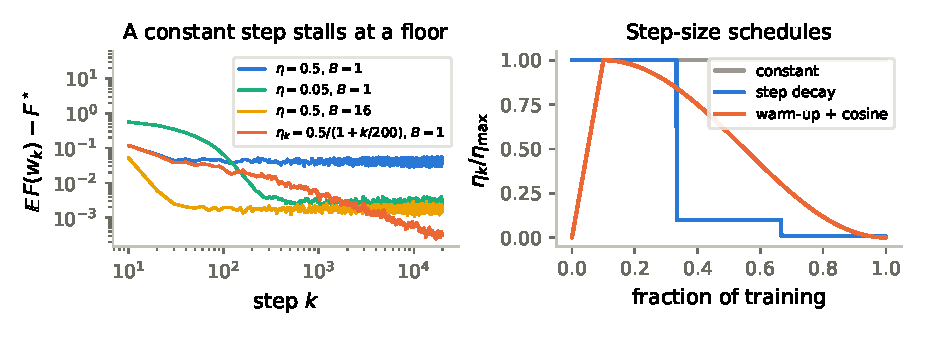
\includegraphics[width=0.84\textwidth]{noise_floor.pdf}
\end{center}
\footnotesize
\alert{Left.} The same least-squares problem, now from $w_0=0$; mean of 20 runs.
\begin{itemize}
\item $\eta=0.5$, $B=1$ stalls at $4.1\cdot10^{-2}$. Dividing $\eta$ by 10 lowers the floor to $2.8\cdot10^{-3}$ and slows the start; $B=16$ lowers it to $1.8\cdot10^{-3}$ at 16 times the cost per step.
\item The values $\frac{\eta}{4B}\operatorname{tr}\Sigma$ are $2.7\cdot10^{-2}$, $2.7\cdot10^{-3}$ and $1.7\cdot10^{-3}$; the floor of the theorem is $2L/\mu=7.4$ times larger.
\item A step $\eta_k\sim1/k$ keeps descending, like $1/k$ \citep{bottou2018}.
\end{itemize}
\alert{Right.} Hence schedules: large steps first, small steps at the end, such as warm-up and cosine decay \citep{loshchilov2017}. Decaying $\eta$ and increasing $B$ lower the same ratio $\eta/B$ \citep{smith2018}.
\end{frame}


% =========================================================================
\begin{frame}{The digit classifier with different batch sizes}
\begin{center}
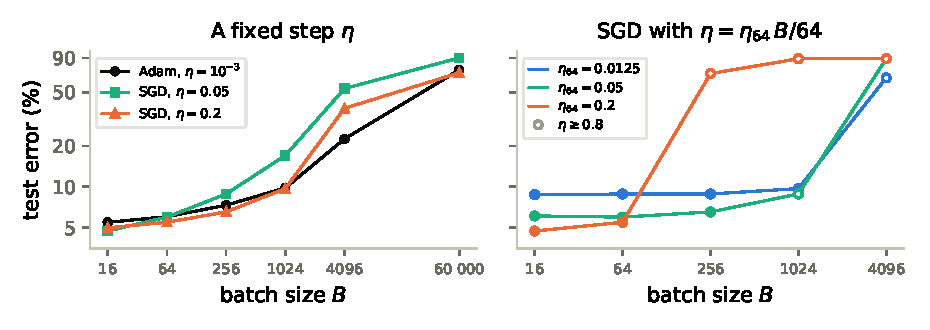
\includegraphics[width=0.82\textwidth]{mnist_batch_size.pdf}
\end{center}
\footnotesize
Data, network, loss and five epochs of the baseline; only the optimizer changes. One run per point: other seeds move the accuracy by up to one point.
\begin{itemize}
\item \alert{Left: a fixed step.} Five epochs are $5N/B$ steps, from $18\,750$ ($B=16$) to $5$ ($B=N$). Adam: $94.6\%$, then the baseline $94.0\%$, down to $26.8\%$.
\item \alert{Right: $\eta\propto B$}, the linear scaling rule \citep{goyal2017}: the same time $k\eta=5N\,\eta/B$ and the same noise $\eta/B$. SGD with $\eta_{64}=0.0125$ gives $91.3$, $91.2$, $91.2$ and $90.3\%$ for $B=16$ to $1024$.
\item The rule ends where the step is unstable: with $\eta\ge0.8$ (hollow) five of six runs fail. The noise scales with $B$, a stability limit such as $\eta<2/L$ does not.
\end{itemize}
\end{frame}


% =========================================================================
\begin{frame}{Inside the fourth box: training is a feedback loop}
\begin{columns}[c]
\begin{column}{0.50\textwidth}
\centering
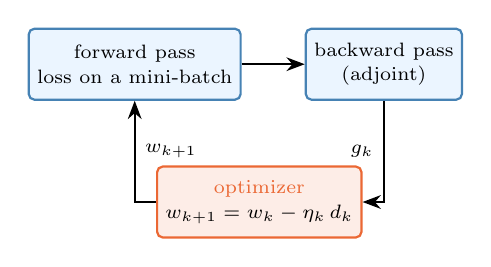
\begin{tikzpicture}[>=Stealth, thick,
  block/.style={draw=boxframe, fill=boxbg, rounded corners=2pt, align=center, font=\scriptsize, inner sep=3pt, minimum height=9mm, minimum width=17mm}]
  \node[block] (net) {forward pass\\[1pt] loss on a mini-batch};
  \node[block, right=8mm of net] (back) {backward pass\\[1pt] (adjoint)};
  \node[block, draw=ctrl, fill=ctrl!12] (opt) at ($(net)!0.5!(back)+(0,-1.75)$) {\ctrl{optimizer}\\[1pt] $w_{k+1}=w_k-\eta_k\,d_k$};
  \draw[->] (net) -- (back);
  \draw[->] (back.south) |- node[pos=0.25, left, font=\scriptsize]{$g_k$} (opt.east);
  \draw[->] (opt.west) -| node[pos=0.75, right, font=\scriptsize]{$w_{k+1}$} (net.south);
\end{tikzpicture}

\medskip
\scriptsize The optimizer observes the gradient $g_k$ and decides the new weights $w_{k+1}$: it is the \ctrl{controller} of the loop.
\end{column}
\begin{column}{0.50\textwidth}
\footnotesize
Lecture 01 distinguished two kinds of control.

\smallskip
\alert{Open loop}, $u=u(t)$: decided in advance.
\begin{itemize}
\item a \emph{schedule} $\eta_k$: step decay, cosine, warm-up
\end{itemize}

\smallskip
\alert{Closed loop}, $u=F(x(t))$: computed from what is observed.
\begin{itemize}
\item line search: shrink $\eta$ until $F$ decreases
\item Adam: rescale each coordinate by a running average of $|g_k|$
\item early stopping: stop when the validation loss rises
\end{itemize}
\end{column}
\end{columns}

\medskip
\footnotesize
``Tuning'' is the design of this controller, and not only by analogy. In the modified equation of a one-dimensional quadratic, the steps $\eta\,u_t$, $u_t\in[0,1]$, that minimize the expected loss at a time $T$ solve an optimal control problem. The solution is a \alert{feedback law}: the full step while the loss dominates the noise, then a decay like $1/t$ \citep{li2017}.
\end{frame}


% =========================================================================
\begin{frame}{Where $g_k$ comes from: backpropagation is an adjoint equation}
\small
A network is a discrete dynamical system: layer $k$ is the time, the depth $L$ the horizon.
\[
x_{k+1}=f_k(x_k,w_k),\quad k=0,\dots,L-1,\qquad x_0=x,\qquad\text{loss }\ell(x_L).
\]
\begin{mathbox}{Backpropagation}
\textbf{Forward.} Compute and store $x_0,\dots,x_L$.\qquad \textbf{Backward.} Set $p_L=\nabla\ell(x_L)$ and
\[
p_k=\big(\partial_xf_k(x_k,w_k)\big)^{\!\top}p_{k+1},\qquad
\nabla_{w_k}\ell=\big(\partial_wf_k(x_k,w_k)\big)^{\!\top}p_{k+1}.
\]
\end{mathbox}
\footnotesize
\begin{itemize}
\item One forward and one backward pass give the derivative with respect to \alert{all} the parameters, at the cost of a few evaluations of the network \citep{rumelhart1986}.
\item $p_k$ is the \alert{adjoint state}: a linear system running backward, like $\varphi'=-A^*\varphi$ behind the control of lecture 01 (notebooks 03 and 07).
\item $p_0=\big(\partial_xf_0\big)^{\!\top}\cdots\big(\partial_xf_{L-1}\big)^{\!\top}p_L$ is a \alert{product of $L$ Jacobians}. Whether it vanishes or explodes is a question of stability: appendix.
\end{itemize}
\nbref{09 \S5, 13 \S5}
\end{frame}


% #########################################################################
% PART 5: THE LOOP AT SCALE
% #########################################################################

% Part 5: the loop at scale.  Overfitting, parameters against data, the implicit bias of
% gradient descent, double descent, scaling laws, the bitter lesson, the edge of stability
% and spectral bias.  Figures: figures/part5_surprises.py and figures/part5_scale.py.

% =========================================================================
\section{The loop at scale}

\begin{frame}{The whole loop: fitting is not learning}
\centering
\loopdiagram{5}

\vspace{1mm}
\begin{columns}[c]
\begin{column}{0.40\textwidth}
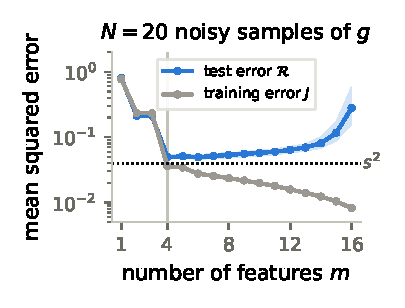
\includegraphics[width=\textwidth]{overfitting_classical.pdf}
\end{column}
\begin{column}{0.60\textwidth}
\footnotesize
The loop makes the empirical risk $F$ small. We want the population risk $\Risk$ small. The \alert{generalization gap} is $\Risk(\hat w)-F(\hat w)$.

\smallskip
\alert{Figure.} Least squares, $m$ polynomials, $s=0.2$.
\begin{itemize}
\item Best at $m=4$: $\Risk=0.049$, for a noise level $s^2=0.04$.
\item At $m=16$: $F=0.008$ and $\Risk=0.28$. The model fits the noise: \alert{overfitting}.
\end{itemize}
\end{column}
\end{columns}
\footnotesize\raggedright
\alert{Why.} With $m\le N$ linearly independent features and uncorrelated noise of variance $s^2$, the fitted values are a projection of rank $m$ of the labels. On average over the noise,
\[
F(\hat w)=b_m^2+s^2\Big(1-\frac mN\Big),\qquad
F'(\hat w)=b_m^2+s^2\Big(1+\frac mN\Big),
\]
with $F'$ on fresh labels at the same inputs and $b_m^2$ the mean squared distance, at the samples, from $g$ to their span. The gap $2s^2m/N$ counts \alert{parameters per sample}.
\nbref{09 \S6--8}
\end{frame}


% =========================================================================
\begin{frame}{How many parameters, how many data?}
\begin{columns}[T]
\begin{column}{0.55\textwidth}
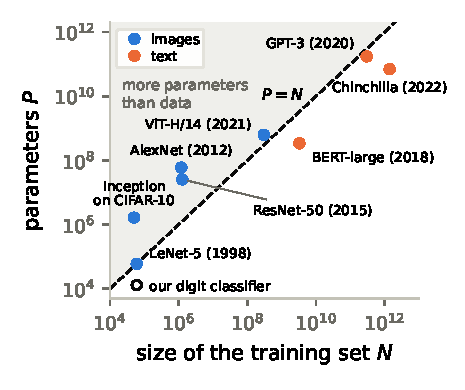
\includegraphics[width=\textwidth]{parameters_vs_data.pdf}

\scriptsize $N$ counts labelled examples: images, or the words or tokens of the training text. Counts from \citep{brown2020,devlin2019,dosovitskiy2021,he2016,hoffmann2022,krizhevsky2012,lecun1998,zhang2017}.
\end{column}
\begin{column}{0.45\textwidth}
\footnotesize
The classical advice: $P\ll N$.
\begin{itemize}
\item Our digit classifier: $13\,002$ parameters for $60\,000$ images.
\item AlexNet (2012): $6\cdot10^{7}$ parameters for $1.2\cdot10^{6}$ images, $50$ \alert{parameters per image}.
\item Such networks fit their training set \alert{exactly}, even with random labels \citep{zhang2017}. On the true labels they predict well.
\item Language models have fewer parameters than tokens, and do not interpolate: the regime of the scaling laws below.
\end{itemize}

\smallskip
\begin{center}
\alert{With more parameters than data, zero training loss does not determine the model. What does?}
\end{center}
\end{column}
\end{columns}
\end{frame}


% =========================================================================
\begin{frame}{Which interpolant? The implicit bias of gradient descent}
\footnotesize
With $m>N$ parameters, $\Phi w=y$ has infinitely many solutions. The algorithm chooses one: steering a state with the least energy and fitting data with the smallest weights are one problem.
\begin{mathbox}{Proposition (gradient descent selects the minimal-norm solution)}
Let $F(w)=\tfrac12\|\Phi w-y\|^2$ with $\Phi\in\R^{N\times m}$ of rank $N$. Gradient descent from $w_0=0$ with $\eta<2/\|\Phi\|^2$ converges to
$w^\dagger=\Phi^\top\big(\Phi\Phi^\top\big)^{-1}y$, the solution of $\Phi w=y$ of smallest norm.
\end{mathbox}
\emph{Proof.} Every step adds a vector of $\Range\Phi^\top$, so $w_k\in\Range\Phi^\top$. The residual $r_k=\Phi w_k-y$ obeys $r_{k+1}=(I-\eta\,\Phi\Phi^\top)\,r_k\to0$. The only solution in $\Range\Phi^\top$ is $w^\dagger$; any other is $w^\dagger+n$ with $n\in\ker\Phi\perp\Range\Phi^\top$, hence longer. \hfill$\square$

\medskip
\begin{mathbox}{The same formula as the minimal-norm control of lecture 01}
\renewcommand{\arraystretch}{1.25}
\begin{tabularx}{\linewidth}{@{}>{\raggedright\arraybackslash}X >{\raggedright\arraybackslash}X@{}}
\textbf{Control:} \ $u=L_T^*\big(L_TL_T^*\big)^{-1}d$ & \textbf{Interpolant:} \ $w=\Phi^\top\big(\Phi\Phi^\top\big)^{-1}y$ \\
$\Gram_T=L_TL_T^*$ invertible: controllable & $\Phi\Phi^\top$ invertible: the data can be fitted \\
cost $\|u\|^2=d^*\Gram_T^{-1}d$ & norm $\|w\|^2=y^\top(\Phi\Phi^\top)^{-1}y$ \\
\end{tabularx}
\end{mathbox}
\end{frame}


% =========================================================================
\begin{frame}{Surprise 1: double descent}
\begin{center}
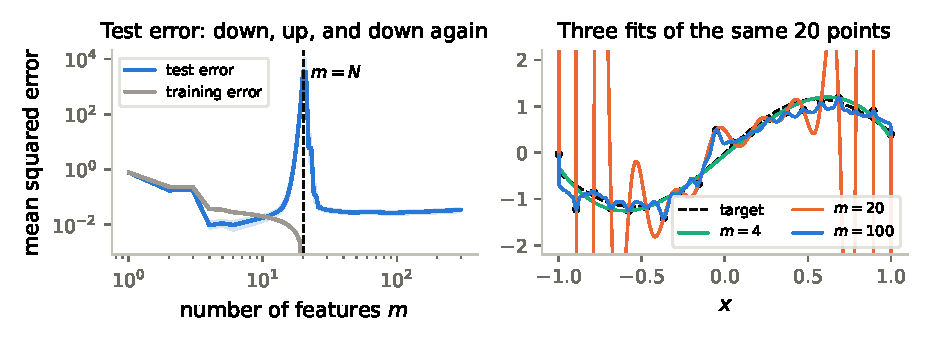
\includegraphics[width=0.74\textwidth]{double_descent.pdf}
\end{center}
\footnotesize
The opening experiment, continued past $m=N$ with the minimal-norm interpolant. The test error is now the distance to $g$: the risk without the noise level $s^2=0.04$.
\begin{itemize}
\item \alert{$m<N$:} the classical regime. Best at $m=4$ (test error $0.009$), then overfitting.
\item \alert{$m=N$:} the interpolating polynomial oscillates wildly: error of order $10^3$.
\item \alert{$m>N$:} the minimal-norm interpolant is tame: test error $0.03$, training error $0$.
\end{itemize}
What matters is \emph{which} interpolant is selected \citep{belkin2019}. Past $m=N$ \alert{more parameters help}: the noise goes into many directions that matter little for prediction \citep{bartlett2020}, a \emph{blessing of dimensionality}, to borrow Donoho's phrase \citep{donoho2000}. Here the second descent stays above the classical optimum; in deep networks it can pass it \citep{nakkiran2021}.
\end{frame}


% =========================================================================
\begin{frame}{Scaling in miniature: more data, more parameters}
\begin{center}
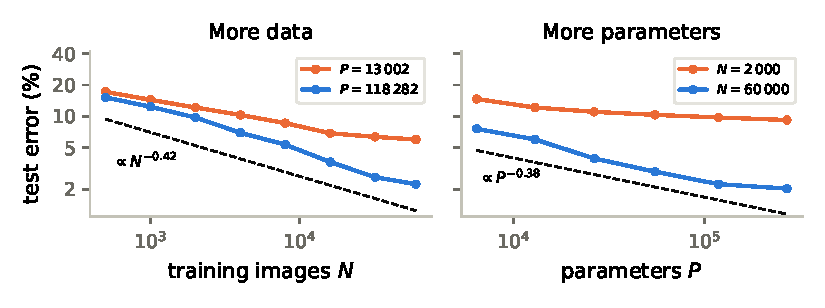
\includegraphics[width=0.77\textwidth]{scaling_mnist.pdf}
\end{center}
\footnotesize
The baseline with $784\to h\to h\to10$ on the first $N$ digits; same loss, same optimizer, $4\,690$ steps, one run per point.
\begin{itemize}
\item \alert{More data.} With $P=118\,282$ the test error falls from $15.2\%$ to $2.2\%$: a fitted exponent $0.42$. With $P=13\,002$, the baseline of the lecture, it flattens at $6\%$: the model is the bottleneck.
\item \alert{More parameters.} With all the images, from $7.6\%$ to $2.0\%$: exponent $0.38$. With $2\,000$ images it flattens above $9\%$: the data are the bottleneck.
\end{itemize}
A toy: two decades at most, single runs. Its shape is the point: \alert{a power law, until the other quantity runs out}.
\end{frame}


% =========================================================================
\begin{frame}{Scaling laws}
\footnotesize
\begin{mathbox}{Scaling laws for language models \citep{kaplan2020}}
Transformers, $768$ to $1.5\cdot10^{9}$ parameters; test loss $L$ in nats per token, $N$ tokens:
\[
L(P)\approx\Big(\frac{P_c}{P}\Big)^{0.076},\qquad L(N)\approx\Big(\frac{N_c}{N}\Big)^{0.095},
\]
each when the other quantity is not the bottleneck.
\end{mathbox}
\begin{itemize}
\item \alert{Small exponents, but predictable.} Ten times the parameters lower the loss by $16\%$, ten times the data by $20\%$; the law in $P$ holds over six orders of magnitude.
\item \alert{Scale matters more than shape:} depth against width has little effect.
\item \alert{Parameters and data grow together.} For a compute budget $C\propto PN$ the best choice is $P\propto C^{0.5}$, $N\propto C^{0.5}$ \citep{hoffmann2022}. Chinchilla ($7\cdot10^{10}$ parameters, $1.4\cdot10^{12}$ tokens) beats Gopher ($2.8\cdot10^{11}$, $3\cdot10^{11}$) for the same compute.
\end{itemize}
These are empirical fits, with more tokens than parameters. The runs behind \citep{hoffmann2022} see less than one pass of their data: every gradient uses fresh samples, and SGD descends the population risk itself (part 4).
\end{frame}


% =========================================================================
\begin{frame}{The bitter lesson}
\footnotesize
\begin{mathbox}{R.~Sutton, \emph{The Bitter Lesson}, 2019 \citep{sutton2019}}
``The biggest lesson that can be read from 70 years of AI research is that general methods that leverage computation are ultimately the most effective, and by a large margin.''
\end{mathbox}
In chess, Go, speech and vision, built-in knowledge helped at first, then lost to search and learning with more computation. Symmetries, he says, should not be built in.

\smallskip
\alert{A tension with parts 1 and 2,} which built knowledge into the loop: Fourier features into the representation, the translation symmetry into the convolution.
\begin{itemize}
\item \alert{With little data the prior wins.} On MNIST the CNN of part 2 beats the MLP.
\item \alert{With much data it need not.} In \citep{dosovitskiy2021}, vision transformers trained on $1.3\cdot10^{6}$ images stay a few points below ResNets of comparable size; pre-trained on $3\cdot10^{8}$ images they pass them: ``large scale training trumps inductive bias''.
\item A prior stands in for data. It is worth most where data are scarce and the knowledge is exact, as with physical laws. Sutton's own example of vision keeps ``the notions of convolution and certain kinds of invariances''.
\end{itemize}
\end{frame}


% =========================================================================
\begin{frame}{Surprise 2: the edge of stability}
\begin{center}
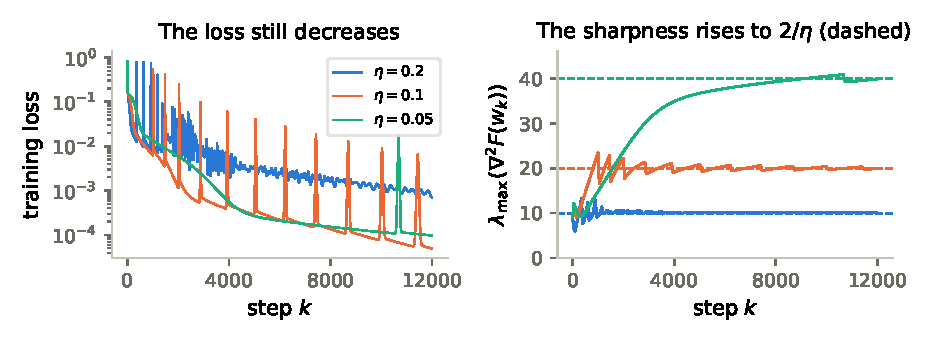
\includegraphics[width=0.84\textwidth]{edge_of_stability.pdf}
\end{center}
\footnotesize
Full-batch gradient descent on $g$: a $\tanh$ network $1\to24\to24\to1$, 40 samples. The \alert{sharpness} is the largest eigenvalue of $\nabla^2F(w_k)$.
\begin{itemize}
\item Lecture 02: on a quadratic, gradient descent is stable if and only if $\eta<2/L$.
\item In a network the curvature is not given. It \alert{rises during training} until it reaches $2/\eta$ and stays there: $10.1$, $20.0$ and $39.5$ for $\eta=0.2$, $0.1$, $0.05$.
\item There the loss is no longer monotone, yet it decreases over long times \citep{cohen2021}.
\end{itemize}
\alert{The step size decides the curvature, not the other way round.} The descent lemma with $\eta\le1/L$ does not describe this regime.
\end{frame}


% =========================================================================
\begin{frame}{Surprise 3: the smooth part is learned first}
\begin{center}
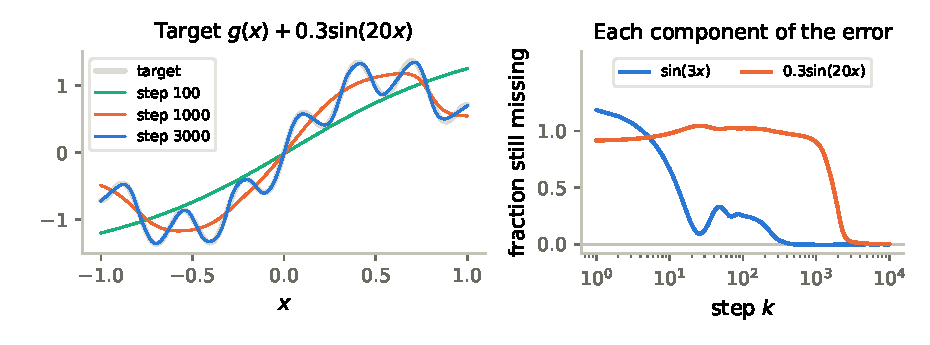
\includegraphics[width=0.78\textwidth]{spectral_bias.pdf}
\end{center}
\footnotesize
The target is now $g(x)+0.3\sin(20x)$; a $\tanh$ network $1\to64\to64\to1$ trained with Adam.
\begin{itemize}
\item After $1000$ steps the slow part is fitted and $90\%$ of the ripple is still missing. The ripple arrives by step $3000$.
\item Networks fit low frequencies first: the \alert{spectral bias} \citep{rahaman2019}. For very wide networks the tangent kernel gives a linear explanation (appendix).
\item Part 1 removed this obstacle by changing the representation of $x$.
\item \alert{Stopping early} then acts as a low-pass filter: one reason why training does not immediately fit the noise.
\end{itemize}
\end{frame}


% #########################################################################
% CLOSING
% #########################################################################

% =========================================================================
\section{Training as a control problem}

\begin{frame}{Training as a control problem}
\footnotesize
\renewcommand{\arraystretch}{1.3}
\begin{tabularx}{\textwidth}{@{}>{\raggedright\arraybackslash}p{0.40\textwidth} >{\raggedright\arraybackslash}X >{\raggedright\arraybackslash}p{0.13\textwidth}@{}}
\toprule
\textbf{Control} & \textbf{Learning} & \textbf{Notebook} \\
\midrule
time $t$, horizon $T$ & layer $k$, depth $L$ & 13 \\
state $x(t)$ & features $x_k$ of one data point & 13 \\
\ctrl{control} $u(t)$ & \ctrl{weights} $(W_k,b_k)$ & 13 \\
one control for many initial states & one network for all training points & 14 \\
adjoint state & backpropagated gradient & 07, 13 \\
control cost $\alpha\!\int\!|u|^2\,dt$ & weight decay & 13 \\
minimal-norm control, Gramian $L_TL_T^*$ & minimal-norm interpolant, Gram matrix $\Phi\Phi^\top$ & 03 \\
friction of an oscillator & momentum & 11 \\
open loop / feedback & schedule / adaptive optimizer & \\
\bottomrule
\end{tabularx}

\medskip
\begin{itemize}
\item Supervised learning with a ResNet or a neural ODE is the \alert{simultaneous control} of $N$ trajectories by one control \citep{e2017,chen2018,ruizbalet2023}.
\item Some rows are identities, others analogies: notebook 19 keeps track of which.
\end{itemize}
\end{frame}


% =========================================================================
\begin{frame}{Open questions}
\small
\begin{itemize}
\item \alert{Why do the solutions found by SGD generalize?} Implicit bias is understood for linear models. For networks there are partial results on flat minima and on the role of the noise, and known counterexamples.
\item \alert{Feature learning.} The kernel regime explains the training of very wide networks, in which the features barely move. Practical networks do learn features. What do they learn, and when?
\item \alert{Grokking.} On small algorithmic tasks a network can reach zero training loss early and generalize only much later \citep{power2022}.
\item \alert{Depth as time.} Very deep residual networks are long-horizon control problems. Does a turnpike property organize their layers \citep{geshkovski2022}? Notebooks 08 and 13.
\item \alert{Constructive training.} Control theory builds explicit controls. Can such constructions replace, or initialize, gradient descent? Notebook 14.
\end{itemize}
\end{frame}


% =========================================================================
\begin{frame}{Key takeaways}
\footnotesize
\begin{enumerate}
\item \alert{Data.} The model sees a representation $\varphi$, and choosing it is modelling. With 16 Fourier harmonics as input, the same network fits the ripple from step 44 instead of step 2350.
\item \alert{Architecture.} An architecture is an assumption on the data, most cleanly a symmetry: a convolutional network with $5\,994$ parameters reads the digits at $98.7\%$, and loses its gain when the pixels are shuffled. Depth composes.
\item \alert{Loss.} The loss decides what is learned: the conditional mean for the squared loss, the conditional law for the log-loss. With a rare class, a weight in the loss is a threshold on the probability.
\item \alert{Optimization.} On fresh samples SGD descends the population risk. It is an Euler--Maruyama scheme of temperature $\eta/B$: near a minimum it stalls at $\tfrac{\eta}{4B}\operatorname{tr}\Sigma$.
\item \alert{At scale.} With more parameters than data the algorithm selects the solution: double descent. Errors fall like power laws in the data and in the parameters. The sharpness settles at $2/\eta$.
\item \alert{Control.} Backpropagation is an adjoint equation, a schedule an open-loop control, an adaptive optimizer a feedback. The Gramian returns in the minimal-norm interpolant and in the noise of SGD.
\end{enumerate}
\end{frame}


% #########################################################################
% ADDITIONAL MATERIAL
% #########################################################################

% =========================================================================
% Additional material: frames of the former Part II of lecture 02 that the four steps do
% not need, kept for questions.
\appendix

\begin{frame}[standout]
Additional material

\medskip
\normalsize Depth, initialization, approximation rates and the tangent kernel
\end{frame}


% =========================================================================
\begin{frame}{Depth in detail: composing the hat function}
\begin{center}
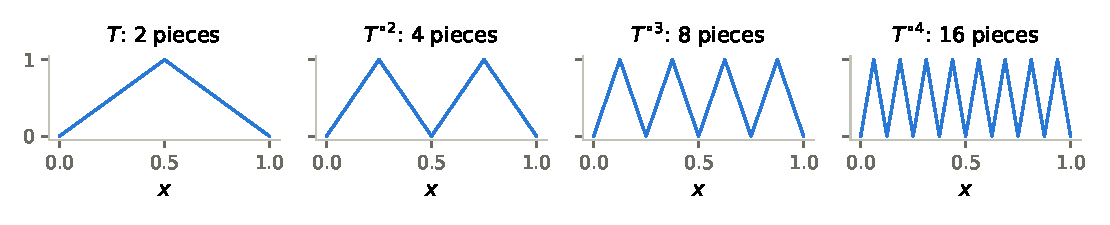
\includegraphics[width=\textwidth]{sawtooth.pdf}
\end{center}
\footnotesize
Courant's hat function takes two ReLU neurons: $T(x)=2\,\sigma(x)-4\,\sigma(x-\tfrac12)$ on $[0,1]$. Composing it $k$ times uses $2k$ neurons in $k$ layers and gives $2^k$ linear pieces.
\begin{mathbox}{Proposition (depth separation)}
A one-hidden-layer ReLU network with $m$ neurons has at most $m+1$ linear pieces: it needs $m\ge2^k-1$ neurons to represent $T^{\circ k}$, where the deep network uses $2k$.
\end{mathbox}
\begin{itemize}
\item Such functions cannot even be \emph{approximated} by much shallower networks unless these are exponentially wide \citep{telgarsky2016}. Applied to the number of ones among $n$ bits, $T^{\circ k}$ is the parity of part 2.
\item $T$ is the \alert{tent map}, a chaotic relative of the logistic map of lecture 01: depth iterates a map, and complexity grows exponentially with time.
\end{itemize}
\end{frame}


% =========================================================================
\begin{frame}{Initialization and depth: a stability problem}
\begin{center}
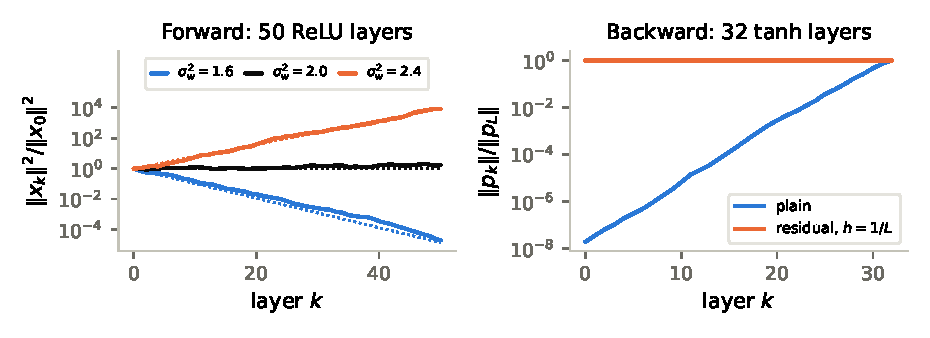
\includegraphics[width=0.80\textwidth]{signal_propagation.pdf}
\end{center}
\footnotesize
\alert{Forward.} ReLU layers $x_{k+1}=\sigma(W_kx_k)$ of width $n$ with $W_{ij}\sim\mathcal N(0,\sigma_w^2/n)$. The ReLU keeps half of a symmetric second moment:
\[
\E\,\|x_{k+1}\|^2=\tfrac12\,\sigma_w^2\,\|x_k\|^2 .
\]
A linear recursion (dotted): $0.8^{50}\approx10^{-5}$ and $1.2^{50}\approx10^{4}$. The choice $\sigma_w^2=2$ sits on the stability boundary \citep{he2015}.

\smallskip
\alert{Backward.} With PyTorch's default initialization, 32 $\tanh$ layers shrink the adjoint by a factor $10^{-8}$. A \alert{residual} layer $x_{k+1}=x_k+h\,\sigma(W_kx_k+b_k)$ has a Jacobian close to the identity, and the adjoint keeps its size \citep{he2016}: the Euler step of lecture 01.
\end{frame}


% =========================================================================
\begin{frame}{How many pieces? Rates and the curse of dimensionality}
\begin{columns}[T]
\begin{column}{0.51\textwidth}
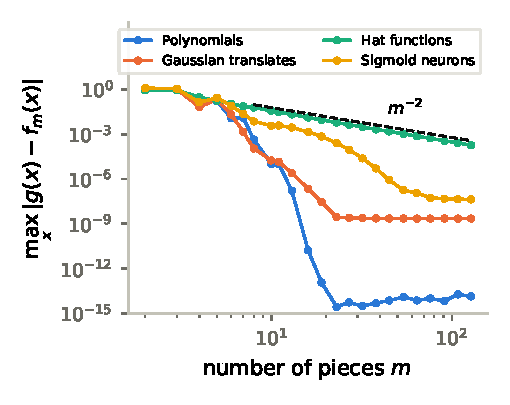
\includegraphics[width=\textwidth]{rates.pdf}

\scriptsize Least-squares fits of $g$ on $[-1,1]$. The flat parts at $10^{-9}$ and $10^{-14}$ are rounding errors.
\end{column}
\begin{column}{0.49\textwidth}
\footnotesize
Density gave no rate. For our analytic target in one dimension:
\begin{itemize}
\item hat functions converge like $m^{-2}$;
\item polynomials converge exponentially fast.
\end{itemize}

\medskip
\alert{In dimension $d$} a mesh of spacing $h$ has $m\approx h^{-d}$ nodes. Hat functions then need
\[
m\approx\varepsilon^{-d/2}\quad\text{pieces for an error }\varepsilon .
\]
With $d=784$ this is hopeless: the \alert{curse of dimensionality}.

\medskip
It is not a defect of hat functions. For targets with $s$ bounded derivatives, no fixed basis of $m$ functions does better than $m^{-s/d}$ in the worst case.
\end{column}
\end{columns}
\end{frame}


% =========================================================================
\begin{frame}{Barron's theorem: why we move the pieces}
\small
\begin{mathbox}{Theorem (Barron, 1993)}
Let $g:\R^d\to\R$ with $C_g=\int_{\R^d}|\omega|\,|\hat g(\omega)|\,d\omega<\infty$. For every $m$ there is a network $f_m$ with one hidden layer of $m$ sigmoid neurons such that, for every probability measure $\mu$ on the ball of radius $r$,
\[
\|g-f_m\|_{L^2(\mu)}\le\frac{2\,r\,C_g}{\sqrt m}.
\]
\end{mathbox}
\begin{itemize}
\item The rate $m^{-1/2}$ \alert{does not depend on the dimension} \citep{barron1993}. The dimension hides in the constant $C_g$.
\item No fixed basis of $m$ functions achieves this uniformly over the same class of targets: there the worst case is of order $m^{-1/d}$.
\item So \alert{the neurons must adapt to $g$}: the inner weights $(a_j,b_j)$ are chosen for each target.
\end{itemize}

\medskip
\begin{center}
\emph{This is why we move the pieces, and accept a non-convex optimization problem.}
\end{center}
\end{frame}


% =========================================================================
\begin{frame}{A linear explanation of spectral bias: the tangent kernel}
\small
Let $r=f(X;w)-y$ be the residual on the training data and $J=\partial_wf(X;w)$ its Jacobian. Along the gradient flow of $\tfrac12\|r\|^2$,
\[
\dot w=-J^\top r\qquad\Longrightarrow\qquad\dot r=J\,\dot w=-J\,J^\top r=-K\,r .
\]
\begin{mathbox}{The kernel regime}
For very wide networks $K=JJ^\top$ barely moves during training \citep{jacot2018}. Then
\[
r(t)=e^{-Kt}\,r(0)=\sum_ie^{-\lambda_it}\,\langle r(0),v_i\rangle\,v_i ,\qquad Kv_i=\lambda_iv_i .
\]
\end{mathbox}
\footnotesize
\begin{itemize}
\item Each eigenvector decays at its own rate, and the smooth ones have the large eigenvalues: \alert{the elongated quadratic of lecture 02, in function space}.
\item $K=JJ^\top$ is a Gram matrix once more. $\lambda_{\min}(K)>0$ drives the training loss to zero, as $\lambda_{\min}(\Gram_T)>0$ gives controllability.
\item In this regime, training is a \emph{linear} dynamical system in the sense of lecture 01. Real networks leave it: their features move.
\end{itemize}
\end{frame}


% =========================================================================
\begin{frame}[allowframebreaks]{References}
\scriptsize
\bibliographystyle{plainnat}
\bibliography{the_training_loop}
\end{frame}

\end{document}
